% !Mode:: "TeX:UTF-8"
\chapter{Inertial Navigation and Integrated Navigation}
\label{cpt:ins}
\thispagestyle{empty}
This chapter introduces the most fundamental techniques of inertial navigation and integrated navigation to the readers. In practice, if you work in the field of traditional navigation, your basic task is to refine details at the level of integrated navigation. However, this book aims to introduce the fusion positioning knowledge of traditional inertial navigation and laser positioning at the beginning of the book.

This section will cover the basics of IMU and satellite positioning. We will discuss the \textbf{measurement model} and \textbf{noise model} of IMU, demonstrating its integration effect. We will find that estimating system state solely based on IMU is not realistic; they tend to diverge quickly (in terms of position) if you use cheap MEMS IMUs. Then we will implement a simple integrated navigation scheme using an error state Kalman filter. It is consistent with the principles of traditional integrated navigation but uses a manifold notation manner and does not introduce complex compensation parameters. You can think of it as an extremely simple integrated navigation scheme. They can achieve integrated navigation functions and can flexibly integrate with other data sources in subsequent chapters. We hope that through this approach, readers can clearly see the differences between traditional and modern theories, providing inspiration for readers in various research directions.

\includepdf[width=\textwidth]{art/ch3.pdf}

\section{Kinematics of IMU Systems}
\label{sec:imu-kinematic}
\subsection{Kinematics}
The \textbf{Inertial Measurement Unit} (IMU) has become very common. IMUs can be found in most electronic devices: vehicles, smartphones, watches, helmets, and even soccer balls. They are small in size and, once installed in a device, can provide effective local motion estimation, enabling various interesting functionalities. In autonomous driving, inertial navigation devices are also fundamental positioning devices. The positioning provided by inertial navigation is basically independent of the external environment and other sensor data, exhibiting high versatility and reliability.

A typical six-axis IMU consists of a \textbf{gyroscope} and an \textbf{accelerometer}. Although they measure the inertia of objects, the means of implementation are diverse, ranging from low-cost MEMS (Micro-electromechanical systems) inertial navigation to expensive fiber-optic gyroscopes (Figure~\ref{fig:real-imus}). Their goal is to accurately measure the inertia of objects. The goal of this book is not to introduce the types and working principles of IMUs themselves\footnote{Readers interested in how IMUs measure angular velocity and acceleration can refer to books that focus more on the manufacturing and measurement principles of IMUs, such as \cite{Qin2014,Yan2019}.}, but to examine their mathematical model properties from the perspective of fusion positioning and state estimation, and further introduce their applications in laser and vision systems.

IMUs are typically installed in a moving system. We infer the state of the object itself by measuring the inertia of the moving carrier. These inertia-related physical quantities are usually not directly position and rotation but rather their differentials. The gyroscope of an IMU can measure the object's \textbf{angular velocity}, while the accelerometer measures the object's \textbf{acceleration}. Internally, they can calculate angular velocity and acceleration based on other physical quantities such as force or time. However, from an external perspective, we only need to be concerned with whether their measurements of angular velocity and acceleration are accurate and the relationship between these quantities and the vehicle's position and orientation.

Based on the kinematics introduced earlier, we can simply write down the kinematic equations in continuous time\footnote{The mathematical symbols in this book are kept simple. We try to avoid adding various subscripts and superscripts, while maintaining consistency throughout the text. However, most of the materials still tend to write out complete symbols with subscripts and superscripts \cite{Huai2018}. This may make the formulae appear more complex, but readers should be able to discern the writing habits of different books.}:

\begin{subequations}\label{eq:motion-equation}
	\begin{align}
		\dot{\bm{R}} &= \bm{R} \boldsymbol{\omega}^\wedge, \quad \text{or} \  \dot{\bm{q}} = \frac{1}{2} 
		\bm{q} \boldsymbol{\omega}, \\
		\dot{\bm{p}} &= \bm{v}, \\
		\dot{\bm{v}} &= \bm{a}.
	\end{align}
\end{subequations}
The rotational part can be represented either by a rotation matrix, as seen in Equation \eqref{eq:rotation-matrix-kinematics}, or by quaternions, as seen in Equation \eqref{eq:quaternion-kinematics}. These physical quantities, when annotated with subscripts, should be denoted as $\bm{R}_{wb}$ and $\bm{p}_{wb}$. Since $\bm{p}_{wb}$ corresponds to the vehicle's world coordinates, after differentiation, it becomes the velocity and acceleration of the vehicle in the world coordinate system, denoted as $\bm{v}_w$ and $\bm{a}_w$. This notation is intuitive, so subsequent text will omit the subscripts related to coordinate systems. Other materials may define variables such as $_w \bm{v}_{wb}$ to distinguish between world-frame velocity and body-frame velocity, but this book uniformly uses quantities in the world frame, with special cases mentioned separately.

The above equations assume that the world frame is fixed, akin to outer space or virtual space. When we do not consider the Earth's rotation, we can simply regard the surface the vehicle travels on as a fixed world coordinate system. In this case, the measured values of IMU, $\tilde{\boldsymbol{\omega}}$ and $\tilde{\bm{a}}$, are the vehicle's own angular velocity and acceleration in the body frame\footnote{We need a notation to distinguish between \textbf{state variables} and \textbf{measurement values}. They can refer to the same physical quantity. However, state variables are estimable and variable, while measurement values are the readings of instruments and are constant. Later text generally uses variables with a tilde to express measurement values, while those without denote state variables.}:
\begin{subequations}\label{key}
	\begin{align}
		\tilde{\bm{a}} &= \bm{R}^\top \bm{a}, \\
		\tilde{\boldsymbol{\omega}} &= \boldsymbol{\omega}.
	\end{align}
\end{subequations}
Note that $\bm{R}^\top$ with the subscript denotes $\bm{R}_{bw}$, which transforms quantities from the world frame to the body frame.

However, real vehicles and robots operate on the surface of the Earth. These systems are influenced by gravity, so we should include gravity in the system equations. In most IMU systems, we can ignore the disturbance caused by the Earth's rotation\footnote{In some high-precision systems, IMUs can measure the Earth's rotation, but in platforms such as vehicles and drones, we usually choose to ignore these physical quantities.}, thus writing the IMU measurements as:
\begin{subequations}\label{eq:3.2}
	\begin{align}
		\tilde{\bm{a}} &= \bm{R}^\top (\bm{a} - \bm{g}), \\
		\tilde{\boldsymbol{\omega}} &= \boldsymbol{\omega}.
	\end{align}
\end{subequations}
Here, $\bm{g}$ represents the gravity of the Earth. Of course, if measuring the object's acceleration in a zero-gravity environment, the gravity term would not appear.

Note that the sign of $\bm{g}$ is related to the definition of the coordinate system. In our coordinate system, both the body frame and the world frame have the $Z$-axis pointing upwards, so $\bm{g}$ typically takes the value $(0, 0, -9.8)^\top$. However, in some books, the $Z$-axis can be defined as pointing towards the center of the Earth, in which case the value of $\bm{g}$ itself or the sign here might be reversed. According to the coordinate system definition in this book, the term in the measurement equation should be $\bm{a}-\bm{g}$.

To aid understanding, readers can also imagine a horizontally placed IMU (see Figure \ref{fig:imu}). If the IMU is stationary, since the measurement of object acceleration is actually obtained by measuring the force applied, the IMU should experience a supporting force in the opposite direction. Therefore, it should measure a gravity in the $-\bm{g}$ direction. If the IMU is flipped upside down, $\bm{R}^\top$ changes, and a positive gravity $\bm{g}$ would be measured. On the other hand, if the IMU is in free fall, the sensors themselves would not detect any external force influence, so $\bm{a}-\bm{g}=\bm{0}$, and the accelerometer should output a zero measurement.

\begin{figure}
	\centering
	\includegraphics[width=\textwidth]{ins/imu.pdf}
	\caption{Illustration of IMU measurements: during free fall, the IMU does not detect any readings; when horizontally placed, the IMU measures gravity in the opposite direction through the supporting force.}
	\label{fig:imu}
\end{figure}

Note that Equation \eqref{eq:3.2} is written under the assumption of \textbf{no noise influence}. If one wants to design a simulation system, equations without noise models can be used. However, actual IMU measurements typically contain noise, so we need to consider the influence of noise.

\subsection{Explanation of IMU Measurements}

Here, we provide some explanations for the IMU measurement equations mentioned earlier, which might be areas where many students encounter issues in engineering practice.

In theory, according to Newton's second law, the force acting on an object is directly proportional to its acceleration, with the coefficient being the object's mass. For an object located in outer space or in free fall, unaffected by external forces, this is indeed the case. We can also imagine an IMU using springs to measure force. In outer space or during free fall, the springs should be in a relaxed state, and no force should be detected. However, most of the time, we are concerned with real moving objects such as vehicles and robots, which mostly operate on the Earth's surface. Due to the Earth's gravitational force, these objects are naturally subjected to an external force $\bm{g}$. If an object is stationary on the Earth's surface, although the net force acting on it is zero, the IMU still naturally detects a supporting force in the opposite direction. At this time, although the object is not accelerating, the IMU can still read the opposite gravity. Hence, we have a $-\bm{g}$ term in the measurement equation. If we consider an IMU in space, we would remove this gravity term from the measurement equation. Alternatively, if the gravity at a particular location differs from elsewhere, we should adjust the value of $\bm{g}$. However, in some materials, gravity is not included in the measurement equation, and real-world IMUs may remove gravity when outputting data. Readers should be aware of such cases.

Furthermore, if the IMU is not placed at the center of the vehicle, when the vehicle rotates and moves, the IMU should also measure the centrifugal force, Coriolis force, and angular acceleration caused by the vehicle's rotation, reflected in the accelerometer readings. Some vehicles also experience various mechanical vibrations, such as suspension systems, moving parts of the vehicle (brushes, rollers, mechanical arms, etc.), which can also affect IMU readings. Therefore, the complete equation should include these terms. However, if all these small terms are included in the subsequent state estimation equations, the equations will become excessively long, which is not conducive to teaching. In practice, these readings themselves are small, and by ensuring that the IMU is installed as close to the vehicle's center as possible, we can avoid the problems caused by misalignment between the IMU and the vehicle's coordinate system. For these reasons, we will continue to use this simplified IMU measurement model in the subsequent discussions.


\subsection{Noise Model in IMU Measurement Equations}
\label{sec:imu-noise}

In most systems, we consider the noise in an Inertial Measurement Unit (IMU) to consist of two parts: \textbf{measurement noise} and \textbf{bias}. Why do we do this? Due to various reasons, even when a vehicle is stationary, the output of angular velocity and acceleration from an IMU may not form a white noise with a mean of $\bm{0}$, but rather have some \textbf{offset}. This offset is caused by the electromechanical measuring devices within the IMU; some IMUs have small offsets while others may have larger ones. Additionally, this offset is also influenced by factors such as temperature and changes over time. Mathematically, we model it and consider \textbf{bias} as a state variable of the system, which undergoes random changes over time. However, readers should understand that this is a \textbf{mathematical model}, not the \textbf{essence of the system}. We do not derive the variation relationship of bias from the mechanical or physical characteristics of the IMU, nor do we physically describe the relationship between IMU bias and temperature, even if such a relationship objectively exists. We simply \textbf{assume} that the mathematical model is such, and then observe if it significantly differs from the actual readings of the IMU device\footnote{Therefore, readers should not assume that there objectively exists a physically measurable quantity termed bias inside the IMU, and then this quantity is superimposed on the measurement values.}. In most systems, such modeling relationships are sufficient. However, if not, we can also add various compensation parameters as needed to accurately describe the variation of bias.

Let the measurement noise of the gyroscope and accelerometer be denoted as $\boldsymbol{\eta}_g, \boldsymbol{\eta}_a$, and let the biases be denoted as $\bm{b}_g, \bm{b}_a$, where the subscript $g$ represents the gyroscope and $a$ represents the accelerometer. Then, these parameters manifest in the measurement equations as follows:
\begin{subequations}\label{eq:imu-measurement}
	\begin{align}
		\tilde{\bm{a}} &= \bm{R}^\top (\bm{a} - \bm{g}) + \bm{b}_a + \boldsymbol{\eta}_a, \\
		\tilde{\boldsymbol{\omega}} &= \boldsymbol{\omega} + \bm{b}_g + \boldsymbol{\eta}_g.
	\end{align}
\end{subequations}

In continuous time, we consider the IMU measurement noise to be a zero-mean white Gaussian process with variances $\mathrm{Cov}(\boldsymbol{\eta}_g)$ and $\mathrm{Cov}(\boldsymbol{\eta}_a)$\footnote{For basic information on Gaussian processes, readers can refer to Section 2.3 in \cite{Barfoot2016}.}. Additionally, we regard the biases as Wiener processes, also known as Brownian motion or random walk. These are common and classical stochastic processes.

A zero-mean white Gaussian process random variable $\bm{w}(t)$ with covariance $\boldsymbol{\Sigma}$ can be expressed as:
\begin{equation}\label{eq:white-gaussian-process}
	\bm{w}(t) \sim \mathcal{GP}(\bm{0}, \boldsymbol{\Sigma} \delta (t-t')),
\end{equation}
where $\boldsymbol{\Sigma}$ is termed the \textbf{energy spectral density matrix}, and $\delta$ denotes the Dirac delta function. The presence of the Dirac delta function enables us to easily derive the IMU measurement noise after discrete-time sampling from the continuous-time Gaussian process. For detailed derivations, please refer to the appendix of \cite{Crassidis2006}, and we will also discuss this in the subsequent sections when introducing the discrete-time model.

On the other hand, a typical random walk process for a bias $\bm{b}$ can be modeled as:
\begin{equation}\label{eq:random-walk}
	\dot{\bm{b}}(t) = \boldsymbol{\eta}_b (t),
\end{equation}
where $\boldsymbol{\eta}_b (t)$ is also a Gaussian process. Therefore, the random walks for $\bm{b}_a$ and $\bm{b}_g$ can be modeled as follows:
\begin{subequations}\label{eq:bias-random-walk}
	\begin{align}
		\dot{\bm{b}}_a (t) &= \boldsymbol{\eta}_{ba}(t) \sim \mathcal{GP}(\bm{0}, 
		\mathrm{Cov}(\boldsymbol{b}_a) \delta (t-t')), \\
		\dot{\bm{b}}_g (t) &= \boldsymbol{\eta}_{bg}(t) \sim \mathcal{GP}(\bm{0}, 
		\mathrm{Cov}(\boldsymbol{b}_g) \delta (t-t')).
	\end{align}
\end{subequations}

If readers are not familiar with stochastic processes, we can also provide an intuitive understanding. Since the covariance of a Gaussian process increases with time, the measurement values of an IMU itself become less accurate as the sampling time increases. Therefore, a higher sampling frequency IMU tends to have higher precision. Meanwhile, the bias part is described by Brownian motion, exhibiting a random walk behavior. In practice, we can think of an IMU's bias starting from some initial value and randomly moving irregularly around it. The larger the magnitude of this movement, the more unstable the bias is. Therefore, a better quality IMU should maintain its bias near the initial value without significant deviation.

\textbf{Random walk} is essentially a stochastic process whose derivative is a Gaussian process. From the perspective of an IMU, since we are concerned with measuring angular velocity and acceleration, the bias part appears as a random walk. However, from a higher-level system perspective, angular velocity is the derivative of angle, and acceleration is the derivative of velocity. So, the IMU's measurement noise can also be interpreted as a \textbf{random walk of angles} and \textbf{random walk of velocities}. Therefore, when encountering the term "random walk," it's important not to only associate it with the bias part, but rather to consider the problem more holistically.

Please note that Gaussian processes and Brownian motion processes mentioned here are \textbf{mathematical models} of IMU measurement data. Mathematical models do not necessarily correspond exactly to the real world. Sometimes, mathematical models are a \textbf{simplification} of reality, which facilitate subsequent algorithmic computations. We should understand this concept. Later on, when we perform linear approximations and retain various first-order terms in many systems, it's based on this \textbf{simplification} mindset. The real measurement noise and bias of IMUs are influenced by many factors such as vehicle vibration, temperature, IMU's own forces, calibration, installation errors, and so on. Modeling them as two stochastic processes is more for the convenience of state estimation algorithm computation, rather than being a perfect, accurate modeling approach. This \textbf{simplify-then-compensate} approach is very common in practice.

\subsection{Discrete-Time Noise Model for IMU}

Although the noise equations for IMUs in continuous time are relatively complex, they simplify significantly in discrete time. In practice, IMUs sample the inertia of moving objects at fixed time intervals, so the data we obtain is always discrete. The complete derivation of the discrete-time model is cumbersome; interested readers can refer to \cite{Crassidis2006}. Here, we only present the conclusions. Because IMU sensors sample at a fixed frequency, let's assume the sampling interval is $\Delta t$. Then, for the noise, the discrete measurement noises of the gyroscope and accelerometer can be simplified as\footnote{Some small terms from \cite{Crassidis2006} are neglected.}:
\begin{subequations}\label{eq:discrete-noise}
	\begin{align}
		\boldsymbol{\eta}_{g}(k) & \sim \mathcal{N}(0, \frac{1}{\Delta t}  \mathrm{Cov}(\boldsymbol{\eta}_g)),
		\\
		\boldsymbol{\eta}_{a}(k) & \sim \mathcal{N}(0,  \frac{1}{\Delta t} \mathrm{Cov}(\boldsymbol{\eta}_a)) .
	\end{align}
\end{subequations}
As for the bias part, it can be written as:
\begin{subequations}\label{eq:discrete-bias}
	\begin{align}
		\bm{b}_g(k+1) - \bm{b}_g(k) &\sim \mathcal{N}(\bm{0}, \Delta t \ \mathrm{Cov}(\bm{b}_g)), \\
		\bm{b}_a(k+1) - \bm{b}_a(k) &\sim \mathcal{N}(\bm{0}, \Delta t \ \mathrm{Cov}(\bm{b}_a)).
	\end{align}
\end{subequations}

Therefore, in discrete-time systems (which is what we usually deal with), both noises are very easy to handle. In many system implementations, even the \textbf{covariance matrices} are not used to express the IMU measurement noise and bias random walk. Instead, they are simply represented as \textbf{diagonal matrices}, effectively ignoring the correlation between different axes. In programming, parameters such as $\sigma_g, \sigma_a$ are often used to express the \textbf{standard deviations} of IMU noise, and parameters $\sigma_{bg}, \sigma_{ba}$ are used to express the \textbf{standard deviations} of bias drift. In this case, the standard deviations of noise in discrete time should be written as:
\begin{subequations}\label{eq:noise-std-dev}
	\begin{align}
		\sigma_{g}(k) &= \frac{1}{\sqrt{\Delta t}} \sigma_g , \quad	\sigma_{a}(k) = \frac{1}{\sqrt{\Delta t}} 
		\sigma_a, \\
		\sigma_{bg}(k) &= \sqrt{\Delta t} \sigma_{bg} , \quad 	\sigma_{ba}(k) = \sqrt{\Delta t} \sigma_{ba} .
	\end{align}
\end{subequations}
When discussing filters and preintegration later on, we will use these symbols to configure the noise conditions of the IMU. Physically, in discrete time, the noise is directly added to the measured physical quantities, making it easy to determine their physical units. The bias in discrete time itself is added to the measured physical quantities, so they share the same units \cite{Woodman2007}.
\begin{equation}\label{eq:physical-units}
	\sigma_g (k) \rightarrow \frac{rad}{s}, \quad \sigma_a(k) \rightarrow \frac{m}{s^2}, \quad 
	\sigma_{bg}(k) \rightarrow \frac{rad}{s}, \quad \sigma_{ba}(k) \rightarrow \frac{m}{s^2}.
\end{equation}
Continuous-time variances need to be multiplied or divided by a square root time unit to obtain discrete variances, so their physical units become:
\begin{equation}\label{eq:physical-units-continuous}
	\sigma_g  \rightarrow \frac{rad}{\sqrt{s}}, \quad \sigma_a \rightarrow \frac{m}{s \sqrt{s}}, \quad 
	\sigma_{bg} \rightarrow \frac{rad}{s \sqrt{s}}, \quad \sigma_{ba} \rightarrow \frac{m}{s^2 \sqrt{s}}.
\end{equation}
Note that units can be converted between similar units, such as radians to degrees, and seconds to minutes or hours, etc. Some materials may use the unit $\frac{1}{\Delta t}$ as $Hz$, so the physical units of the above variables can also be denoted as:
\begin{equation}\label{eq:physical-units-hertz}
	\sigma_g  \rightarrow \frac{rad}{s \sqrt{Hz}}, \quad \sigma_a \rightarrow \frac{m}{s^2 \sqrt{Hz}}, 
	\quad \sigma_{bg} \rightarrow \frac{rad}{s^2 \sqrt{Hz}}, \quad \sigma_{ba} \rightarrow \frac{m}{s^3 
		\sqrt{Hz}}.
\end{equation}

\subsection{IMUs in Reality}
\begin{figure}
	\centering
	\includegraphics[width=0.9\textwidth]{ins/real-imu.pdf}
	\caption{Various IMU Products in Reality}
	\label{fig:real-imus}
\end{figure}


\begin{figure}
	\centering
	\includegraphics[width=1.0\linewidth]{./ins/imu-datasheet-cn.png}
	\caption{Datasheet of Real IMUs \emph{TODO: replace}}
	\label{fig:imu-datasheet}
\end{figure}

Figure~\ref{fig:real-imus} displays examples of typical IMU products. Readers can directly purchase various IMU-related products in most markets, including standalone IMU sensors and integrated products. With the miniaturization of IMUs, many products are also integrated with IMUs internally at the factory. The most common example is our everyday smartphones, which commonly integrate low-cost MEMS IMU devices. In the field of robotics, sensors commonly used in applications such as LiDAR, cameras, etc., are also increasingly integrating ready-made IMUs. During the period of writing this book, many solid-state LiDARs (e.g., DJI Livox series, Ouster OS2), monocular and stereo cameras (e.g., Zed 2, MYNT Eye S) have already provided built-in IMUs as sources of inertial navigation data.

IMU products generally provide their own datasheets to illustrate their data accuracy, stability, and other metrics at the time of manufacture. These metrics can also be used to guide us in adjusting the weights of state estimation algorithms. Figure~\ref{fig:imu-datasheet} shows a typical parameter configuration of an IMU (ADIS 16488). It can be seen that the main parameters relevant to our subsequent algorithms are as follows:

\begin{enumerate}
	\item Measurement noise, which in the entire motion model is regarded as \textbf{angular random walk} and \textbf{velocity random walk}, corresponding to $\sigma_g$ and $\sigma_a$ in the \textbf{continuous-time} noise model. We can also simply refer to them as \textbf{gyroscope white noise} and \textbf{accelerometer white noise}. It can be observed that the specifications of this IMU are 0.66$^\circ/\sqrt{\text{hour}}$ and 0.11$m/s/\sqrt{\text{hour}}$. Intuitively, this can be understood as follows: assuming we have correctly identified the bias, if we integrate this IMU, the standard deviation of its integration error per hour should be 0.66$^\circ$ and $0.11m/s$.
	
	\item Bias instability variance, which is also known as $\sigma_{bg}$ and $\sigma_{ba}$ in the noise model. However, this quantity is usually not directly corresponding in the datasheet and is difficult to measure in practice. The datasheet often provides bias repeatability and bias stability during operation instead. When we first turn on the IMU, we can estimate the bias of the IMU in a static state. The variability of each bias change is described by bias repeatability. On the other hand, if other objective conditions remain unchanged, this boot-up bias will also change to some extent during operation. Its magnitude is described by \textbf{operational bias stability}, which in this datasheet is 14.5$^\circ /\text{hour}$. Intuitively, under ideal conditions, we can assume that the bias of the IMU will remain within this range near the initial bias. However, in reality, IMUs often do not operate under constant temperature conditions, and their bias changes need to be estimated in real time. Overall, we can refer to this specification to set the magnitude of bias instability.\footnote{For detailed definitions of these two values, please refer to "GJB 585A-1998 Inertial Technology Terminology".}
\end{enumerate}


\section{Trajectory Estimation Using IMU}

Previously, we introduced how angular velocity and acceleration are measured in a motion system. This approach is a simulation-based perspective or a description of a known system. In other words, we can first assume what motion the object undergoes and then consider what kind of IMU measurements should be generated under this motion. However, the reality is the opposite. We can read the readings of IMU sensors, but we must infer the motion of the system based on the readings of IMU and other sensors, rather than directly obtaining various velocity and acceleration information of the system.

When there are many sensors, we integrate various sensor data for fusion-based positioning or SLAM, which is the main content of this book. Later, we will discuss the fusion of IMU with RTK, LiDAR, and other systems. In this section, we will first examine how to infer the motion state of the system when only IMU data is available. We will find that this approach is feasible, but a system with only IMU requires double integration of IMU readings, and the existence of measurement errors and biases will cause the state variables to drift quickly.

\subsection{Short-Term Trajectory Estimation Using IMU Data}

We have introduced the kinematic model of the IMU system itself in Section \ref{sec:imu-kinematic}, while the measurement model of the IMU is introduced in Equation \eqref{eq:imu-measurement}. Therefore, by directly substituting the measurement model into the kinematic equation and ignoring the influence of measurement noise, we can obtain the integration model in continuous time:

\begin{subequations}\label{key}
	\begin{align}
		\dot{\bm{R}} &= \bm{R} (\tilde{\boldsymbol{\omega}} - \bm{b}_g )^\wedge, \quad \text{or} \ 
		\dot{\bm{q}} = \bm{q} \left[0, \frac{1}{2} \left( \tilde{\boldsymbol{\omega}} -\bm{b}_g\right) 
		\right], \\
		\dot{\bm{p}} &= \bm{v}, \\
		\dot{\bm{v}} &= \bm{R} (\tilde{\bm{a}} - \bm{b}_a) + \bm{g}.
	\end{align}
\end{subequations}

Sometimes we also refer to $\bm{p}, \bm{v}, \bm{q}$ as the PVQ state. This equation can be integrated from time $t$ to $t+\Delta t$ to derive the state at the next moment:

\begin{subequations}\label{eq:3.14}
	\begin{align}
		\bm{R}(t+\Delta t) &= \bm{R}(t) \mathrm{Exp} \left( (\tilde{\boldsymbol{\omega}}-\bm{b}_g) \Delta 
		t \right),\quad \text{or} \ \bm{q}(t+\Delta t) = \bm{q}(t) \left[ 1, \frac{1}{2} \left( 
		\tilde{\boldsymbol{\omega}} - \bm{b}_g\right) \Delta t\right], \\
		\bm{p}(t+\Delta t) &= \bm{p}(t) + \bm{v} \Delta t + \frac{1}{2} \left(\bm{R}(t)(\tilde{\bm{a}}-\bm{b}_a) 
		\right) \Delta t^2 + \frac{1}{2} \bm{g} \Delta t^2, \\
		\bm{v}(t+\Delta t) &= \bm{v}(t) + \bm{R}(t) (\tilde{\bm{a}} - \bm{b}_a) \Delta t + \bm{g} \Delta t	.
	\end{align}
\end{subequations}

With this equation, we can use the state at one moment plus the IMU data at the next moment to infer the state at the next moment. This approach is generally referred to as \textbf{propagation}. From the perspective of numerical integration\footnote{Readers unfamiliar with numerical computation can refer to \cite{LiQinYang2001}.}, it corresponds to the Euler method in numerical integration (Figure~\ref{fig:integ-method}).

\begin{figure}
	\centering
	\includegraphics[width=1\textwidth]{ins/integ-method.pdf}
	\caption{Schematic diagram of different integration methods. From left to right: start-point integration, mid-point integration, trapezoidal integration, true integration.}
	\label{fig:integ-method}
\end{figure}

Different numerical integration methods vary, with the Euler method being the simplest. The rotation and translation of an object itself are continuous, while the IMU samples at fixed time intervals. During the sampling interval $\Delta t$, there are several approaches to handling the angular velocity and acceleration within this small time frame. The Euler method adopts the simplest approach: it assumes that during the time from $t$ to $t+\Delta t$, the object's angular velocity is entirely equal to $\boldsymbol{\omega}(t)$, and the acceleration is equal to $\bm{a}(t)$. This is equivalent to using the starting point of the interval as the function value for the integration rectangle in numerical integration. Other methods, such as the midpoint method, trapezoidal rule, and higher-order interpolation methods (most notably the Runge-Kutta method \cite{Liu2020}), can also be employed. These methods are not overly complex in practice—they simply replace the measurements in the above equations with interpolated values $\tilde{\boldsymbol{\omega}}, \tilde{\bm{a}}$ for the recursion. Theoretically, the midpoint and trapezoidal methods should be more accurate than the simplest Euler integration, while interpolation methods introduce additional computational overhead. Whether the improvement in accuracy justifies the increased computation depends on the specific application.

The above equations can also be accumulated further, such as from time $i$ to time $j$. We only need to aggregate the IMU readings in between:

\begin{subequations}\label{eq:imu-dead-reckoning}
	\begin{align}
		\bm{R}_j &= \bm{R}_i \prod_{k=i}^{j-1}\mathrm{Exp} \left(\left(\tilde{\boldsymbol{\omega}}_k - 
		\bm{b}_{g,k}\right) \Delta t\right) \quad \text{or}\quad \bm{q}_j = \bm{q}_i \prod_{k=i}^{j-1} \left[1, 
		\frac{1}{2} \left(\tilde{\boldsymbol{\omega}}_k - \bm{b}_{g,k}\right) \Delta t \right], \\
		\bm{p}_j &= \bm{p}_k + \sum_{k=i}^{j-1} \left[\bm{v}_k \Delta t + \frac{1}{2} \bm{g} \Delta t^2\right] + 
		\frac{1}{2} \sum_{k=i}^{j-1} \bm{R}_k \left(\tilde{\bm{a}}_k - \bm{b}_{a,k} \right) \Delta t^2, \\
		\bm{v}_j &= \bm{v}_i + \sum_{k=i}^{j-1}\left[ \bm{R}_k\left(\tilde{\bm{a}}_k - \bm{b}_{a,k} \right) 
		\Delta t+ \bm{g} \Delta t  \right].
	\end{align}
\end{subequations}

Note that we have not yet considered the influence of noise. In Chapter~\ref{cpt:preinteg}, we will further examine the impact of measurement noise and bias noise on IMU integration. Here, we focus only on its recursive form. Observe that the above equations are essentially \textbf{incremental}: each $\bm{R}_k, \bm{v}_k$ can serve as the computation result for the next time step. Therefore, in code implementation, when an IMU frame arrives, we can use the result from the previous frame to compute the recursion for the next frame, without waiting for all data to arrive before performing the accumulation as per the formula. For rotation, there is no fundamental difference between using quaternions or rotation matrices, though the rotation matrix representation is more concise mathematically and does not require frequent normalization. In this chapter, we retain both notations for readers to compare. However, in subsequent chapters, we will primarily use the rotation matrix representation.

\subsection{Code Experiment for IMU Recursion}
Below, we conduct an experiment to demonstrate how to use IMU data for trajectory propagation. Without external observations, we can only use Equation (\ref{eq:imu-dead-reckoning}) to perform double integration and obtain the position and attitude information of the moving object. This integration typically diverges rapidly, making IMU unsuitable for standalone dead reckoning. Our experiment will illustrate this.

\begin{lstlisting}[language=c++,caption=ch3/imu_integration.h]
class IMUIntegration {
	public:
	IMUIntegration(const Vec3d& gravity, const Vec3d& init_bg, const Vec3d& init_ba)
	: gravity_(gravity), bg_(init_bg), ba_(init_ba) {}
	
	text
	// Add IMU reading
	void AddIMU(const IMU& imu) {
		double dt = imu.timestamp_ - timestamp_;
		if (dt > 0 && dt < 0.1) {
			// Assume IMU time interval is between 0 and 0.1
			p_ = p_ + v_ * dt + 0.5 * gravity_ * dt * dt + 0.5 * (R_ * (imu.acce_ - ba_)) * dt * dt;
			v_ = v_ + R_ * (imu.acce_ - ba_) * dt + gravity_ * dt;
			R_ = R_ * Sophus::SO3d::exp((imu.gyro_ - bg_) * dt);
		}
		
		// Update time
		timestamp_ = imu.timestamp_;
	}
	
	/// Compose NavState
	NavStated GetNavState() const { return NavStated(timestamp_, R_, p_, v_, bg_, ba_); }
	
	SO3 GetR() const { return R_; }
	Vec3d GetV() const { return v_; }
	Vec3d GetP() const { return p_; }
	
	private:
	// Accumulated quantities
	SO3 R_;
	Vec3d v_ = Vec3d::Zero();
	Vec3d p_ = Vec3d::Zero();
	
	double timestamp_ = 0.0;
	
	// Biases, set externally
	Vec3d bg_ = Vec3d::Zero();
	Vec3d ba_ = Vec3d::Zero();
	
	Vec3d gravity_ = Vec3d(0, 0, -9.8);  // Gravity
};
\end{lstlisting}

This function implements a simple IMU integrator that continuously reads IMU data and provides its integration results. We have prepared some sensor data for readers in data/ch3/ (which will also be used in later chapters). Readers can select any trajectory segment and run the following program to observe the IMU integration results.

\begin{lstlisting}[language=c++,caption=ch3/run_imu_integration.cc]
sad::TxtIO io(FLAGS_imu_txt_path);

// In this experiment, we assume biases are known
Vec3d gravity(0, 0, -9.8); // Gravity direction
Vec3d init_bg(00.000224886, -7.61038e-05, -0.000742259);
Vec3d init_ba(-0.165205, 0.0926887, 0.0058049);

sad::IMUIntegration imu_integ(gravity, init_bg, init_ba);

sad::ui::PangolinWindow ui;
ui.Init();

/// Record results
auto save_result = [](std::ofstream& fout, double timestamp, const Sophus::SO3d& R, const Vec3d& v,
const Vec3d& p) {
	auto save_vec3 = [](std::ofstream& fout, const Vec3d& v) { fout << v[0] << " " << v[1] << " " << v[2] << " "; };
	auto save_quat = [](std::ofstream& fout, const Quatd& q) {
		fout << q.w() << " " << q.x() << " " << q.y() << " " << q.z() << " ";
	};
	
	text
	fout << std::setprecision(18) << timestamp << " " << std::setprecision(9);
	save_vec3(fout, p);
	save_quat(fout, R.unit_quaternion());
	save_vec3(fout, v);
	fout << std::endl;
};

std::ofstream fout("./data/ch3/state.txt");
io.SetIMUProcessFunc([&imu_integ, &save_result, &fout, &ui](const sad::IMU& imu) {
	imu_integ.AddIMU(imu);
	save_result(fout, imu.timestamp_, imu_integ.GetR(), imu_integ.GetV(), imu_integ.GetP());
	ui.UpdateNavState(imu_integ.GetNavState());
	usleep(1e2);
}).Go();

ui.Quit();
\end{lstlisting}

This program stores the integration results in ch3/state.txt. Note that this book frequently uses C++ lambda functions for flexible function calls. Here, TxtIO reads and parses sensor data from text files, then executes callbacks for various sensors as predefined. Since programs in different chapters process this sensor data differently, the callback portion is implemented using lambda functions.

Now, execute this program:
\begin{lstlisting}[language=sh, caption=Terminal input:]
bin/run_imu_integration
\end{lstlisting}

It will display the vehicle's real-time position in the UI. However, this program will quickly diverge, and the vehicle will disappear off the screen edge. After the program ends, we can run the plotting script to visualize the trajectory:
\begin{lstlisting}[language=sh, caption=Terminal input:]
python3 scripts/plot_ch3_state.py data/ch3/state.txt
\end{lstlisting}

\begin{figure}
	\centering
	\includegraphics[width=1\textwidth]{ins/ch3-imu-integ-ui.png}
	\caption{IMU integration results displayed in the UI}
	\label{fig:ch3-imu-integ-ui}
\end{figure}

The vehicle motion in the UI is shown in Figure~\ref{fig:ch3-imu-integ-ui}, and the trajectory plotting result is shown in Figure~\ref{fig:ch3-imu-integ}. We observe that the attitude, expressed in quaternions, remains relatively stable overall. The data source is an onboard IMU, with the $q_y, q_z$ components of the quaternion attitude remaining near zero. However, the displacement quickly diverges. Due to the lack of external observations, the velocity state soon becomes uncontrollable, far exceeding the vehicle's actual speed (this is a low-speed vehicle under 25 km/h), causing the position estimate to diverge to an extremely large value. Readers can also try other datasets, all of which will diverge rapidly.

\begin{figure}
	\centering
	\includegraphics[width=1\textwidth]{ins/ch3-imu-integ.pdf}
	\caption{Results of IMU integration}
	\label{fig:ch3-imu-integ}
\end{figure}

Later, we will discuss how to fuse IMU data with other sensor data to obtain more accurate state estimates. In traditional navigation, the primary fusion method for IMU is integration with satellite navigation, forming what is known as a GINS (GNSS-INS) system.

\section{Satellite Navigation}
Satellite navigation (Global Navigation Satellite System, GNSS) is another primary source of positioning information for outdoor vehicles. While the internal principles of satellite navigation are highly complex, its output is remarkably simple. That said, if we dissect practical systems down to their fundamental principles, we quickly become overwhelmed by engineering details. Even seemingly simple systems like microcontrollers can appear extremely intricate when explained at the circuit level. Therefore, we will not introduce GNSS systems starting from rocket or satellite launches but instead approach the topic from a more practical perspective: What information can satellite navigation provide to an autonomous vehicle?

The answer to this question is straightforward. During normal operation, satellite navigation can provide all the positioning information a vehicle needs, including its position, attitude, velocity, and other physical quantities. Readers might then ask: Can autonomous driving be achieved using satellite positioning alone? To answer this, we must consider several factors:

\begin{enumerate}
	\item Does the positioning accuracy of GNSS meet the requirements?
	
	\item Is the positioning frequency of GNSS sufficient for downstream applications?
	
	\item How reliable is GNSS positioning? Can it be used in all weather conditions and locations?
	
\end{enumerate}

In reality, GNSS encompasses many subtypes, and there is no uniform answer to these questions. Some GNSS methods offer high accuracy but require the object to remain stationary for a period (typically over ten minutes). Others provide better dynamic positioning but require the prior setup of one or more base stations. Almost all GNSS systems face the challenge of being "weather-dependent"—their stability is influenced by the environment, structures, obstructions, and even the day's weather. This makes satellite navigation in the autonomous driving industry often accurate enough but difficult to control in terms of reliability.

Classification and Providers of GNSS
Broadly speaking, GNSS systems determine their position by measuring the distance to satellites orbiting the Earth, primarily through time-of-flight calculations. A satellite signal carries a transmission timestamp when emitted, and the GNSS receiver records its arrival time. By comparing these timestamps, the distance to each satellite can be estimated. The main differences among GNSS systems and measurement methods lie in how they reduce timing errors. From this perspective, GNSS can essentially be viewed as a high-precision timekeeping system.

\begin{figure}
	\centering
	\includegraphics[width=0.7\textwidth]{ins/rtk-receivers.pdf}
	\caption{Various GNSS/RTK receivers.}
	\label{fig:rtk-receivers}
\end{figure}

Currently, satellite signals received worldwide primarily come from four systems:

\begin{enumerate}
	\item GPS (Global Positioning System, USA)
	
	\item BDS (Beidou Navigation Satellite System, China)
	
	\item GLONASS (Russia)
	
	\item GALILEO (European Union)
\end{enumerate}


Each system has deployed 20 to 30 satellites in space. Systems that directly use these satellites for positioning are typically called standalone GNSS\footnote{GNSS systems are continuously evolving. Due to historical reasons, the term "GPS" was commonly used in the past, but most literature now distinguishes between GPS and GNSS.}. Most ground-based GNSS receivers can access signals from multiple satellite systems, choosing either a single source or combining multiple sources. Standalone GNSS typically provides positioning accuracy within a few meters. Most mobile devices use standalone GNSS for navigation (Figure~\ref{fig:rtk-receivers}).

The final accuracy of satellite positioning is affected by many factors, from the satellite's electromagnetic signals to transmission delays and receiver clock errors. Various correction techniques have been developed to mitigate these errors, such as PPP (Precise Point Positioning) and RTK (Real-Time Kinematic), which continue to improve positioning accuracy. These technologies are extensive, but this book focuses on the user perspective rather than the development side.

By 2023, GNSS positioning has evolved from ~10-meter accuracy to real-time centimeter-level precision, becoming widely accessible. In China, providers like Qianxun, Hezhong, and Xunteng offer extensive and affordable satellite positioning services, increasingly integrated into consumer devices like smartphones and vehicles.

For autonomous vehicles, the most commonly used satellite positioning technologies include:

Standalone GNSS: Traditional meter-level satellite positioning, cost-effective and widely used in phones and car systems. While sufficient for road-level navigation\footnote{Autonomous driving typically requires lane-level navigation, which identifies the vehicle's specific lane, offering greater stability than road-level navigation.}, its accuracy struggles to distinguish between parallel roads (e.g., highways vs. service roads).

RTK Positioning: To address signal transmission errors, differential positioning was developed, where a ground-based reference station with known coordinates corrects the vehicle's GNSS signals. RTK, based on carrier-phase differential technology, uses one or more base stations to provide real-time corrected positioning.

Many companies now offer RTK services for autonomous driving, deploying extensive base station networks and using 4G/5G to deliver real-time vehicle positions. In favorable conditions, RTK alone can enable autonomous driving. Some providers combine RTK with inertial navigation for enhanced reliability.

\subsection{Practical RTK Installation and Data Reception}
As the saying goes, "seeing is believing." Below we present some actual RTK data (the same applies to GNSS data) used in autonomous driving applications.

RTK receivers are typically installed on vehicle rooftops in disc-shaped configurations (often affectionately called "mushroom heads"). A single mushroom head can provide precise satellite positioning. When two receivers are configured in a \textbf{dual-antenna} setup, the vehicle's real-time heading can be calculated based on the positional difference between the two antennas.

\begin{figure}
	\centering
	\includegraphics[width=0.7\textwidth]{ins/apollo-rtk.pdf}
	\caption{A dual-antenna RTK installation configuration from Baidu Apollo's development kit.}
	\label{fig:apollo-rtk}
\end{figure}

Figure~\ref{fig:apollo-rtk} demonstrates a practical dual-antenna RTK installation on a vehicle. With the vehicle body removed, we can clearly observe the installation positions of various sensors. This vehicle features two RTK mushroom heads - one at the front and another at the rear - aligned along the vehicle's longitudinal axis. Other vehicles may employ horizontal or lateral dual-antenna configurations.

In dual-antenna systems, we generally follow these conventions:
\begin{enumerate}
	\item One antenna is designated as the \textbf{primary} antenna, representing the vehicle's position.
	\item The \textbf{secondary} antenna's position is subtracted from the primary's to obtain the directional vector between them, from which the vehicle's heading angle (primarily yaw) can be derived.
	\item For left-right installations, the left antenna is typically designated as primary.
	\item For front-rear installations, the rear antenna is usually primary.
\end{enumerate}

However, these are merely conventional designations - the two antennas are fundamentally identical and their roles could be reversed.

\begin{figure}
	\centering
	\includegraphics[width=0.7\textwidth]{ins/rtk-antenna.pdf}
	\caption{Various dual-antenna RTK installation configurations: left-right, front-rear, and diagonal.}
	\label{fig:rtk-antenna}
\end{figure}

Several key considerations for dual-antenna systems include:
\begin{itemize}
	\item To accurately measure vehicle angles, the two antennas should be placed as far apart as possible\footnote{Both antennas' positions are subject to measurement noise. Greater separation reduces the noise's impact on angle calculations.}.
	\item The distance between dual antennas is called the RTK \textbf{baseline}\footnote{The term "baseline" is widely used across different sensors (e.g., RTK baseline, stereo camera baseline). Readers need not concern themselves with potential connections between these usages.}.
	\item As a sensor system, the RTK's installation position on the vehicle can be described by extrinsic parameters represented by a transformation matrix.
	\item Since dual antennas are typically coplanar, the rotational extrinsic parameters can be described by a single angle called the \textbf{installation yaw angle} (antenna angle), while the translational parameters are called \textbf{installation offset} (antenna position). These parameters are usually determined during structural design.
\end{itemize}

Satellite positioning systems universally output object positions in latitude and longitude coordinates. This output format is tied to Earth's fixed coordinate systems, unlike LiDAR or visual positioning systems where coordinate frames can be arbitrarily defined. Additionally, dual-antenna RTK angle measurements follow conventional definitions. We will first introduce common global coordinate systems before processing actual RTK data.
\subsection{Common World Coordinate Systems}
Various world coordinate systems are widely used in the physical world. Below we briefly introduce their definitions.

\subsubsection{Geographic Coordinate System}
\begin{figure}
	\centering
	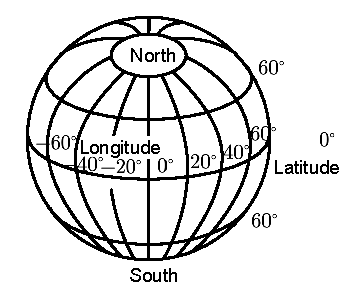
\includegraphics[width=0.4\textwidth]{ins/latlon.pdf}
	\caption{Schematic diagram of latitude-longitude coordinate system}
	\label{fig:latlon}
\end{figure}

The most common coordinate system on Earth is the \textbf{latitude-longitude} coordinate system, also known as the \textbf{Geographic Coordinate System} (see Figure~\ref{fig:latlon}). Combined with altitude, it forms the latitude-longitude-altitude (LLA) coordinate system. Latitude and longitude divide the Earth's surface uniformly: longitude ranges 180 degrees east and west from the prime meridian, while latitude ranges 90 degrees north and south from the equator. Both values are expressed in degrees or radians. Altitude can be either elevation above sea level or geodetic height relative to a reference surface.

While intuitive and globally applicable (being the default for many mapping systems), latitude-longitude coordinates become cumbersome for autonomous driving applications at city-scale or smaller areas. Building-level coordinates typically require 8-9 decimal places, and the nonlinear conversion to metric units (where 1 degree longitude corresponds to 0 meters at the poles but over 100 km at the equator) motivates the use of local coordinate systems.

\subsubsection{UTM Coordinate System}
The Universal Transverse Mercator (UTM) system projects the WGS84 ellipsoid Earth onto a transverse cylinder, divided into 60 longitudinal and 20 latitudinal zones with numeric and alphabetic labels respectively. While roughly uniform in angular distribution, metric distances vary due to Earth's curvature, with significant distortion excluding polar regions beyond 80° latitude.

Within each zone:
\begin{itemize}
	\item Easting coordinates reference a central meridian (assigned x=500,000m), increasing eastward
	\item Northing coordinates measure distance from the equator
	\item The resulting \textbf{ENU} (East-North-Up) system follows right-hand convention
	\item Alternative \textbf{NED} (North-East-Down) configurations also exist
\end{itemize}

UTM advantages include metric compatibility with sensors, though zone boundaries require special handling. Note:
\begin{enumerate}
	\item A 0.9996 scale factor corrects projection distortion
	\item ENU/NED systems have opposite Z-axis orientations affecting angle definitions
	\item Maximum easting span is ~667 km per zone
\end{enumerate}

This metric local frame facilitates autonomous vehicle operations while maintaining global reference.

\subsection{Display of RTK Measurements}
Many RTK and integrated navigation manufacturers can output coordinates in user-selected coordinate systems, with the most basic being the latitude-longitude coordinates measured by the RTK receiver. Below we demonstrate how to convert RTK's latitude-longitude coordinates to metric UTM coordinates while using a dual-antenna configuration to determine the vehicle's heading angle. Here we disregard the vehicle's pitch and roll, treating them as zero. Thus, although the vehicle outputs \textbf{4-DOF coordinates}, under the assumption of zero pitch and roll, the RTK output can also be considered as a 6-DOF pose transformation, i.e., an $\mathrm{SE}(3)$ pose.

We continue using the data from the previous section. This data consists of IMU, RTK, and wheel speed measurements located in the `data/ch3/` directory. Readers can open these files with a text editor, with the format as follows:

\begin{lstlisting}[language=sh, caption=Example data file]
	GNSS 1571900872.47168827 30.0011840411666668 117.97859182983332 305.98748779296875 
	330.047799999999995 1
	ODOM 1571900872.50085688 0 0
	IMU 1571900872.56527948 -0.000740019602845583204 -0.000471238898038460995 
	6.98131700797720067e-06 0.362519161666666645 -0.0608012299999999908 
	9.82135997500000002
\end{lstlisting}

Each line in the file represents a measurement, with the prefix "GNSS", "IMU", or "ODOM" indicating the record type. For GNSS measurements, each line contains: timestamp, latitude, longitude, altitude, heading angle, and heading validity flag. For IMU or wheel speed measurements, the readings from the accelerometer, gyroscope, and wheel speed sensors are provided. The GNSS positioning here is provided by the Qianxun FindCM solution, with a nominal accuracy of 2 cm in fixed solution mode.

Since the algorithm for converting latitude-longitude to UTM coordinates is complex and not the focus of this book, we use an open-source conversion method from the `thirdparty/utm_convert` directory\footnote{See: \url{https://github.com/hobu/mgrs}}. We've added a wrapper function to conveniently compute the $\mathrm{SE}(3)$ pose corresponding to GNSS measurements. The conversion code is as follows:

\begin{lstlisting}[language=c++,caption=ch3/utm\_convert.cc]
bool LatLon2UTM(const Vec2d& latlon, UTMCoordinate& utm_coor) {
	long zone = 0;
	char char_north = 0;
	long ret = Convert_Geodetic_To_UTM(latlon[0] * math::kDEG2RAD, latlon[1] * math::kDEG2RAD, &zone, &char_north,
	&utm_coor.xy_[0], &utm_coor.xy_[1]);
	utm_coor.zone_ = (int)zone;
	utm_coor.north_ = char_north == 'N';
	
	return ret == 0;
}

bool ConvertGps2UTM(GNSS& gps_msg, const Vec2d& antenna_pos, const double& antenna_angle, const Vec3d& map_origin) {
	/// Convert latitude-longitude-altitude to UTM
	UTMCoordinate utm_rtk;
	if (!LatLon2UTM(gps_msg.lat_lon_alt_.head<2>(), utm_rtk)) {
		return false;
	}
	utm_rtk.z_ = gps_msg.lat_lon_alt_[2];
	
	/// Convert GPS heading to radians
	double heading = 0;
	if (gps_msg.heading_valid_) {
		heading = (90 - gps_msg.heading_) * math::kDEG2RAD;  // Convert from NED to ENU
	}
	
	/// Transform from TWG to TWB
	SE3 TBG(SO3::rotZ(antenna_angle * math::kDEG2RAD), Vec3d(antenna_pos[0], antenna_pos[1], 0));
	SE3 TGB = TBG.inverse();
	
	/// Subtract map origin if specified
	double x = utm_rtk.xy_[0] - map_origin[0];
	double y = utm_rtk.xy_[1] - map_origin[1];
	double z = utm_rtk.z_ - map_origin[2];
	SE3 TWG(SO3::rotZ(heading), Vec3d(x, y, z));
	SE3 TWB = TWG * TGB;
	
	gps_msg.utm_valid_ = true;
	gps_msg.utm_.xy_[0] = TWB.translation().x();
	gps_msg.utm_.xy_[1] = TWB.translation().y();
	gps_msg.utm_.z_ = TWB.translation().z();
	
	if (gps_msg.heading_valid_) {
		// Construct pose with rotation
		gps_msg.utm_pose_ = TWB;
	} else {
		// Construct SE3 with only translation
		// Note: When installation offset exists, the actual vehicle pose cannot be derived
		gps_msg.utm_pose_ = SE3(SO3(), TWB.translation());
	}
	
	return true;
}
\end{lstlisting}

The latitude-longitude to UTM conversion is handled by the library function, while we need to transform the UTM coordinates from the GNSS frame to the vehicle's observed pose, considering the RTK's extrinsic parameters. The dual-antenna RTK installation used in this section is shown in Figure~\ref{fig:dual-rtk-coor}, where the blue axes $x_B, y_B, O_B$ represent the vehicle body frame, and the red axes $x_G, y_G, O_G$ represent the GNSS receiver frame.

Mathematically, we can treat the RTK's UTM coordinate reading as $\bm{T}_{WG}$, where $W$ represents the world frame and $G$ represents the GNSS receiver frame. To facilitate subsequent fusion localization, we transform it to $\bm{T}_{WB}$, where $B$ is the vehicle body frame. Thus, the extrinsic parameters between the GNSS receiver and the vehicle can be described by either $\bm{T}_{GB}$ or $\bm{T}_{BG}$.

\begin{figure}
	\centering
	\includegraphics[width=0.3\textwidth]{ins/dual-rtk-coor.pdf}
	\caption{RTK installation configuration used in this book's example. Subscript $G$ denotes the GNSS receiver frame, while $B$ denotes the vehicle body frame. The primary antenna is located at the right rear of the vehicle, and the secondary antenna at the front left.}
	\label{fig:dual-rtk-coor}
\end{figure}

In the calibration parameters, we specify the installation offset $\bm{a}_t$ as the vector from $O_B$ to $O_G$ expressed in the $B$ frame, which essentially corresponds to the translational component of $\bm{T}_{BG}$. Simultaneously, the installation angle $a_{\theta}$ is defined as the rotation angle from the $x$-axis of the $B$ frame to the $x$-axis of the $G$ frame. Substituting $\bm{a}_t$ and $a_{\theta}$ into $\bm{T}_{BG}$, we obtain:

\begin{equation}\label{key}
	\bm{T}_{BG} = \begin{bmatrix}
		\bm{R}_Z (a_{\theta}) & \bm{a}_t \\
		\bm{0}^\top & 1
	\end{bmatrix},
\end{equation}

where $\bm{R}_Z$ represents the rotation matrix about the $Z$-axis.

It's important to note that this definition of \textbf{installation angle} and \textbf{installation offset} is intuitive but not unique. The specific definition should prioritize operational convenience. These parameters could alternatively be defined in the opposite direction, as long as calibration personnel can measure them easily. We typically align mathematical notation with practical conventions rather than forcing real-world operations to conform to mathematical definitions. While calibration personnel might struggle to directly measure $\bm{R}_{BG}$ or $\bm{t}_{BG}$, they can easily measure the connection between two points or the angle between two lines.

The transformation matrix $\bm{T}_{WB}$ from the vehicle body frame to the world frame can be derived from RTK measurements and its extrinsic parameters:

\begin{equation}\label{key}
	\bm{T}_{WB} = \bm{T}_{WG} \bm{T}_{GB}.
\end{equation}

Expanding the rotation and translation components yields:

\begin{equation}\label{key}
	\bm{R}_{WB} = \bm{R}_{WG} \bm{R}_{GB}, \quad \bm{t}_{WB} = \bm{R}_{WG} \bm{t}_{GB} + \bm{t}_{WG}.
\end{equation}

An important consideration: even with known RTK extrinsic parameters $\bm{t}_{GB}$, determining the vehicle coordinates $\bm{t}_{WB}$ requires knowledge of the RTK orientation $\bm{R}_{WG}$. In a single-antenna configuration with non-zero installation offset $\bm{t}_{GB}$, \textbf{the vehicle's world coordinates cannot be precisely determined when the vehicle orientation is unknown}. However, in state estimation algorithms where the vehicle attitude $\bm{R}_{WB}$ is estimated, we can use $\bm{R}_{WB} \bm{R}_{BG}$ as the current $\bm{R}_{WG}$.

Additionally, the conversion program handles the transformation between \textbf{ENU} (East-North-Up) and \textbf{NED} (North-East-Down) coordinate systems. Different RTK manufacturers may output angles according to their predefined schemes, potentially causing inconsistencies in angle definitions. This book uses UTM coordinates with east and north as $XY$ axes (ENU frame), while the RTK manufacturer outputs NED coordinates. The former uses east as zero degrees, while the latter uses north as zero degrees with opposite rotation direction. Therefore, an azimuth angle $h$ in the NED frame converts to angle $h'$ in the ENU frame as:

\begin{equation}\label{key}
	h' = \pi/2 - h.
\end{equation}

The code above implements this angle conversion.

We then write a program to convert GNSS readings from the data file into poses and write them to an output file. Readers can use Python scripts to plot the entire GNSS trajectory. Simultaneously, we display the RTK poses in real-time graphical interfaces, allowing immediate visualization of current position and orientation.

\subsection{RTK Measurement Visualization}
Many RTK and integrated navigation manufacturers can output coordinates in user-selected coordinate systems, with the most basic output being the latitude-longitude coordinates measured by the RTK receiver. Below we demonstrate how to convert RTK's latitude-longitude coordinates to metric UTM coordinates while using a dual-antenna configuration to determine the vehicle's heading angle.

\begin{lstlisting}[language=c++,caption=ch3/process\_gnss.cc]
DEFINE_string(txt_path, "./data/ch3/10.txt", "Input data file path");

// Parameters specific to the provided dataset
DEFINE_double(antenna_angle, 12.06, "RTK antenna installation angle (degrees)");
DEFINE_double(antenna_pox_x, -0.17, "RTK antenna installation offset X");
DEFINE_double(antenna_pox_y, -0.20, "RTK antenna installation offset Y");

/**
* This program demonstrates GNSS data processing
* We convert raw GNSS readings into 6-DOF poses for subsequent processing
* Requires UTM conversion, RTK antenna extrinsics, and coordinate transformation
*
* Results are saved to file and visualized using Python scripts
*/

int main(int argc, char** argv) {
	sad::TxtIO io(fLS::FLAGS_txt_path);
	
	std::ofstream fout("./data/ch3/gnss_output.txt");
	Vec2d antenna_pos(FLAGS_antenna_pox_x, FLAGS_antenna_pox_y);
	
	auto save_result = [](std::ofstream& fout, double timestamp, const SE3& pose) {
		auto save_vec3 = [](std::ofstream& fout, const Vec3d& v) { 
			fout << v[0] << " " << v[1] << " " << v[2] << " "; 
		};
		auto save_quat = [](std::ofstream& fout, const Quatd& q) {
			fout << q.w() << " " << q.x() << " " << q.y() << " " << q.z() << " ";
		};
		
		fout << std::setprecision(18) << timestamp << " " << std::setprecision(9);
		save_vec3(fout, pose.translation());
		save_quat(fout, pose.unit_quaternion());
		fout << std::endl;
	};
	
	std::shared_ptr<sad::ui::PangolinWindow> ui = nullptr;
	if (FLAGS_with_ui) {
		ui = std::make_shared<sad::ui::PangolinWindow>();
		ui->Init();
	}
	
	bool first_gnss_set = false;
	Vec3d origin = Vec3d::Zero();
	io.SetGNSSProcessFunc([&](const sad::GNSS& gnss) {
		sad::GNSS gnss_out = gnss;
		if (sad::ConvertGps2UTM(gnss_out, antenna_pos, FLAGS_antenna_angle)) {
			if (first_gnss_set == false) {
				origin = gnss_out.utm_pose_.translation();
				first_gnss_set = true;
			}
			gnss_out.utm_pose_.translation() -= origin;
			
			save_result(fout, gnss_out.unix_time_, gnss_out.utm_pose_);
			ui->UpdateNavState(
			sad::NavStated(gnss_out.unix_time_, gnss_out.utm_pose_.so3(), 
			gnss_out.utm_pose_.translation()));
			
			usleep(1e4);
		}
	}).Go();
	
	if (ui) {
		while (!ui->ShouldQuit()) {
			usleep(1e5);
		}
		ui->Quit();
	}
	
	return 0;
}
\end{lstlisting}

The program converts RTK readings to UTM poses, removes the origin offset, writes to a text file, and displays in UI. To run:

\begin{lstlisting}[language=sh, caption=Terminal command:]
	bin/process_gnss --txt_path ./data/ch3/10.txt
\end{lstlisting}

The converted 6-DOF coordinates are saved in data/ch3/gnss_output.txt. Visualization scripts:

\begin{lstlisting}[language=sh, caption=Terminal command:]
	python3 scripts/plot_ch3_gnss_2d.py ./data/ch3/gnss_output.txt 
\end{lstlisting}

Figure~\ref{fig:gnss-traj} shows 2D and 3D trajectory plots. Observations:
\begin{itemize}
	\item RTK provides excellent horizontal trajectory accuracy
	\item Vertical measurements show noticeable noise and errors
	\item The example shows good GNSS conditions; other datasets include challenging segments
\end{itemize}

\begin{figure}
	\centering
	\includegraphics[width=1.0\textwidth]{ins/gnss-traj.pdf}
	\caption{2D and 3D views of GNSS trajectory}
	\label{fig:gnss-traj}
\end{figure}

The real-time display (Figure~\ref{fig:process-gnss}) shows:
\begin{itemize}
	\item Proper vehicle orientation (X-forward, Y-left, Z-up) when RTK heading is valid
	\item Noticeable instability in angle measurements compared to position
	\item Position jitter during heading outages due to incomplete pose solution
\end{itemize}

\begin{figure}
	\centering
	\includegraphics[width=1.0\textwidth]{ins/ch3-process-gnss.png}
	\caption{Real-time GNSS trajectory visualization}
	\label{fig:process-gnss}
\end{figure}

Note: This section only uses RTK-provided position and heading. Some RTK/INS systems output additional IMU data (angular/linear velocity), but we focus on fundamental principles here.

\section{Implementing Integrated Navigation Using Error-State Kalman Filter}
The RTK device provides us with a somewhat unstable pose observation source. We can directly treat it as an observation input for a positioning filter. In this section, we will combine RTK with IMU using an extended Kalman filter to form a traditional integrated navigation algorithm for subsequent algorithm comparisons. Strictly speaking, what we present to readers is the \textbf{Error-State Kalman Filter} (ESKF). The ESKF finds extensive applications ranging from GINS integrated navigation to visual SLAM\cite{Kleinert2010,Li2013,Davison2003} and extrinsic calibration\cite{Kelly2011,Mirzaei2008}. 

Why do we need ESKF? What's the difference between ESKF and EKF? We'll start from the motivation level. This progressive approach from simple to complex can also help readers better understand the development process of various algorithms.

\subsection{Mathematical Derivation of ESKF}
We have previously introduced the observation model of IMU devices. Now we need to treat IMU as the motion model and GNSS observations as the measurement model to derive the complete filter. This is not particularly difficult.

We define the state variables as:
\begin{equation}\label{key}
	\bm{x} = [\bm{p}, \bm{v}, \bm{R}, \bm{b}_g, \bm{b}_a, \bm{g}]^\top,
\end{equation}
where all variables default to subscript $()_{WB}$, with $\bm{p}$ representing translation, $\bm{v}$ velocity, $\bm{R}$ rotation, $\bm{b}_g, \bm{b}_a$ biases, and $\bm{g}$ gravity. According to the kinematic equations \eqref{eq:motion-equation} we introduced earlier and substituting IMU measurements, the continuous-time motion equations for the state variables are:
\begin{subequations}\label{eq:ekf-continous}
	\begin{align}
		\dot{\bm{p}} &= \bm{v}, \\
		\dot{\bm{v}} &= \bm{R} (\tilde{\bm{a}} - \bm{b}_{a} - \boldsymbol{\eta}_a) + \bm{g}, \\
		\dot{\bm{R}} &= \bm{R} \left( \tilde{\boldsymbol{\omega}} - \bm{b}_{g} - \boldsymbol{\eta}_g 
		\right)^\wedge, \\
		\dot{\bm{b}}_{g} & = \boldsymbol{\eta}_{bg}, \\
		\dot{\bm{b}}_{a} & = \boldsymbol{\eta}_{ba}, \\ 
		\dot{\bm{g}} &= \bm{0}.
	\end{align}
\end{subequations}

To predict the covariance in the EKF prediction step, we need to linearize these equations. Theoretically, the discrete-time linearized form is:
\begin{equation}\label{key}
	\bm{x}_{k+1} = \bm{f} (\bm{x}_k) + \bm{F} \mathrm{d} \bm{x} + \bm{w},
\end{equation}
where $\bm{F} = \left. \frac{\partial \bm{f}}{\partial \bm{x}} \right|_{\bm{x}_{k}}$ is the coefficient matrix. However, we encounter a practical problem: on one hand, $\bm{F}$ needs to compute the derivative of the rotation matrix $\bm{R}$ relative to some perturbation, and without introducing tensors, we cannot express the derivative of a matrix with respect to a vector. Traditional algorithms often compromise by using Euler angles or four scalars of quaternions as state variables\cite{crassidis2006sigma}, but this approach cannot elegantly utilize methods on manifolds. On the other hand, if we consider integrating inertial navigation systems with satellite navigation systems, the translation variables in $\bm{x}$ should use a global coordinate system. This makes the numerical values in $\bm{x}$ very large, potentially exceeding the effective digit range of floating-point numbers in some scenarios, leading to common computational failures like "large number swallowing small number" in numerical calculations\cite{bonnans2006numerical}.

This leads us to consider: can we avoid directly using $\bm{x}$ and $\bm{P}$ to express the mean and covariance of the state when deriving the motion and observation equations? Can we use the \textbf{update quantity} from the original Kalman filter to derive these two equations? Recall the observation part of the Kalman filter:
\begin{equation}\label{key}
	\bm{x}_k = \bm{x}_{k, \text{pred}} + \bm{K}_k \underbrace{(\bm{z}_k - \bm{H}_k \bm{x}_{k, \text{pred}})}_{\text{update quantity}}.
\end{equation}

In the context of manifolds, the update quantity on the right side should be a vector in the tangent space, and the addition in the middle should be the generalized addition of the manifold and the exponential map of the tangent space. However, we can also treat the update quantity (or error state) as the state variable of the filter to derive the motion and observation models. This leads to the \textbf{Error-State Kalman Filter}. Furthermore, not just for translation and rotation, we express all states in terms of error states, which is the typical approach of ESKF.

The ESKF is widely used in many traditional and modern systems, serving both as a filter for integrated navigation and for implementing complex systems like LIO and VIO\cite{Xu2021,xu2021fast, Bloesch2017}. Compared to traditional KF, the advantages of ESKF can be summarized as follows\cite{Madyastha2011}:
\begin{enumerate}
	\item In handling rotation, ESKF state variables can use minimal parameter representation, i.e., using three-dimensional variables to express rotation increments. These variables lie in the tangent space, which is a vector space. Traditional KF requires quaternions (4D) or higher-dimensional variables (rotation matrices, 9D) to express the state, or must use representations with singularities (Euler angles).
	\item ESKF always operates near the origin, far from singular points, making it more numerically stable and avoiding issues where linearization approximations become inadequate due to operating too far from the working point.
	\item The ESKF state quantities are small, making their second-order variables relatively negligible. Most Jacobian matrices become very simple under small quantities, sometimes even replaceable by identity matrices.
	\item The kinematics of error states are also smaller compared to the original state variables (kinematics of small quantities), allowing us to return the update part to the original state variables.
\end{enumerate}
In ESKF, we typically refer to the original state variables as \textbf{nominal state variables} and the state variables in ESKF as \textbf{error state variables}. The sum of nominal and error state variables is called the \textbf{true value}. By handling noise in the error state variables, we can consider the equations for nominal state variables as noise-free. This approach may seem complex initially, but separating the noise makes the nominal state equations more concise. The filter itself primarily needs to consider how the error state evolves, is observed, and finally filtered, with minimal relation to the nominal state.

The ESKF workflow is as follows: When IMU measurement data arrives, we integrate it into the nominal state variables. Since this approach doesn't account for noise, the results naturally drift quickly, so we treat the error component as error variables. During motion, the nominal state propagates with IMU data, while the error state grows due to Gaussian noise. At this point, the mean and covariance of ESKF's error state describe the specific magnitude of error state expansion (treated as a Gaussian distribution)\footnote{However, as we'll see later, since all noise terms are zero-mean white noise, the mean of the error state remains zero in the motion equations, only the covariance increases.}. Additionally, ESKF's update process relies on sensor observations beyond IMU. During updates, we use sensor data to update the \textbf{posterior} mean and covariance of the error state. We can then \textbf{merge} this error into the nominal state variables and reset ESKF to zero, completing one predict-update cycle.

Let's derive the two processes of ESKF. We define the true state of ESKF as: $\bm{x}_t = [\bm{p}_t, \bm{v}_t, \bm{R}_t, \bm{b}_{at}, \bm{b}_{gt}, \bm{g}_t]^\top$. The subscript $t$ denotes $\text{true}$, i.e., the true state. This state changes over time and can be denoted as $\bm{x}_t(t)$. In continuous time, we record IMU readings as $\tilde{\boldsymbol{\omega}}, \tilde{\bm{a}}$, allowing us to write the relationship between state variable derivatives and observations:

\begin{subequations}\label{eq:eskf-true-state}
	\begin{align}
		\dot{\bm{p}}_t &= \bm{v}_t, \\
		\dot{\bm{v}}_t &= \bm{R}_t (\tilde{\bm{a}} - \bm{b}_{at} - \boldsymbol{\eta}_a) + \bm{g}_t, \\
		\dot{\bm{R}}_t &= \bm{R}_t \left( \tilde{\boldsymbol{\omega}} - \bm{b}_{gt} - \boldsymbol{\eta}_g \right)^\wedge, \\
		\dot{\bm{b}}_{gt} &= \boldsymbol{\eta}_{bg}, \\
		\dot{\bm{b}}_{at} &= \boldsymbol{\eta}_{ba}, \\ 
		\dot{\bm{g}}_t &= \bm{0}.
	\end{align}
\end{subequations}

This is consistent with Equation \eqref{eq:ekf-continous} mentioned earlier. Note that including gravity $\bm{g}$ mainly facilitates determining the IMU's initial attitude. If we don't express gravity in the state equation, we must determine the IMU's initial orientation $\bm{R}(0)$ beforehand to perform subsequent calculations. In this case, the IMU's attitude is described relative to the initial horizontal plane. By explicitly expressing gravity, we can set the IMU's initial attitude as the identity matrix $\bm{R}=\bm{I}$, treating the gravity direction as a measure of the IMU's current attitude relative to the horizontal plane. Both methods are feasible, but separately expressing gravity makes initial attitude representation simpler and increases some linearity\cite{Lupton2009}.

If we organize observations and noise into a vector, we can express the above in matrix form. However, such a matrix would contain many zero entries without significant simplification over the current form, so we'll continue using these expanded equations. Next, we derive the error state equations. First, define the error state variables as:

\begin{subequations}\label{eq:eskf-true-to-error}
	\begin{align}
		\bm{p}_t &= \bm{p} + \delta \bm{p}, \\
		\bm{v}_t &= \bm{v} + \delta \bm{v}, \\
		\bm{R}_t &= \bm{R} \delta \bm{R} \quad \text{or} \ \bm{q}_t = \bm{q} \delta \bm{q}, \\
		\bm{b}_{gt} &= \bm{b}_g + \delta \bm{b}_g, \\
		\bm{b}_{at} &= \bm{b}_a + \delta \bm{b}_a, \\
		\bm{g}_t &= \bm{g} + \delta \bm{g}.
	\end{align}
\end{subequations}

The terms without subscripts are the \textbf{nominal state variables} in Equation (\ref{eq:eskf-true-state}). The kinematic equations for nominal state variables are identical to the true values, except they \textbf{ignore noise} (since noise is considered in the error state equations). For the rotation part, $\delta \bm{R}$ can be represented by its Lie algebra $\mathrm{Exp}(\delta \boldsymbol{\theta})$, requiring Equation (c) to be expressed in exponential form.

For error state Equations (a,d,e,f), taking time derivatives on both sides easily yields corresponding derivative expressions:

\begin{subequations}
	\begin{align}
		\delta \dot{\bm{p}} &= \delta \bm{v}, \\
		\delta \dot{\bm{b}_g} &= \boldsymbol{\eta}_{bg}, \\
		\delta \dot{\bm{b}_a} &= \boldsymbol{\eta}_{ba}, \\
		\delta \dot{\bm{g}} &= \bm{0}.
	\end{align}
\end{subequations}

Equations (b) and (c) are slightly more complex due to their relationship with $\delta \bm{R}$, and we provide their separate derivation below.

\subsubsection{Error State Rotation Term}
Taking the time derivative of both sides of Equation (\ref{eq:eskf-true-to-error})(c) yields:

\begin{equation}\label{eq:eskf-3.19}
	\begin{aligned}
		\dot{\bm{R}}_t &= \dot{\bm{R}} \mathrm{Exp} (\delta \boldsymbol{\theta}) + \bm{R} 
		\dot{\mathrm{Exp}(\delta \boldsymbol{\theta})},  \\
		&\buildrel{\ref{eq:eskf-true-state}(c)}\over=  \bm{R}_t \left( \tilde{\boldsymbol{\omega}} - 
		\bm{b}_{gt} - \boldsymbol{\eta}_g \right) ^\wedge.
	\end{aligned}
\end{equation}

Note that the term $\dot{\mathrm{Exp}(\delta \boldsymbol{\theta})}$ on the right side satisfies:
\begin{equation}
	\dot{\mathrm{Exp}(\delta \boldsymbol{\theta})} = \mathrm{Exp}(\delta \boldsymbol{\theta}) \delta 
	\dot{\boldsymbol{\theta}}^\wedge.
\end{equation} 

Thus, the first expression in \eqref{eq:eskf-3.19} can be written as:
\begin{equation}\label{key}
	\dot{\bm{R}} \mathrm{Exp} (\delta \boldsymbol{\theta}) + \bm{R} \dot{\mathrm{Exp}(\delta 
		\boldsymbol{\theta})} = \bm{R} (\tilde{\boldsymbol{\omega}}-\bm{b}_g)^\wedge 
	\mathrm{Exp}(\delta \boldsymbol{\theta}) + \bm{R} \mathrm{Exp}(\delta \boldsymbol{\theta} ) 
	\delta \dot{\boldsymbol{\theta}}^\wedge.
\end{equation}

While the second expression becomes:
\begin{equation}\label{key}
	\begin{aligned}
		\bm{R}_t \left( \tilde{\boldsymbol{\omega}} - \bm{b}_{gt} - \boldsymbol{\eta}_g \right)^\wedge 
		&= \bm{R}  \mathrm{Exp} (\delta \boldsymbol{\theta}) \left( \tilde{\boldsymbol{\omega}} - 
		\bm{b}_{gt} - \boldsymbol{\eta}_g \right)^\wedge.
	\end{aligned}
\end{equation}

By comparing these two expressions, moving $\delta \dot{\boldsymbol{\theta}}^\wedge$ to one side, canceling $\bm{R}$ on both sides, and organizing similar terms, we obtain:
\begin{equation}
	\begin{aligned}
		\mathrm{Exp} (\delta \boldsymbol{\theta}) \delta \dot{\boldsymbol{\theta}}^\wedge &= 
		\mathrm{Exp} (\delta \boldsymbol{\theta}) \left( \tilde{\boldsymbol{\omega}} - \bm{b}_{gt} - 
		\boldsymbol{\eta}_g \right)^\wedge - (\tilde{\boldsymbol{\omega}}-\bm{b}_g)^\wedge 
		\mathrm{Exp}(\delta \boldsymbol{\theta}).
	\end{aligned}
\end{equation}

Noting that $\mathrm{Exp}(\delta \boldsymbol{\theta})$ itself is an $\mathrm{SO}(3)$ matrix, we utilize the adjoint property of $\mathrm{SO}(3)$:
\begin{equation}\label{key}
	\boldsymbol{\phi}^\wedge \bm{R} = \bm{R} (\bm{R}^\top \boldsymbol{\phi})^\wedge
\end{equation}
to interchange $\mathrm{Exp}(\delta \boldsymbol{\theta})$ above:
\begin{equation}\label{key}
	\begin{aligned}
		\mathrm{Exp} (\delta \boldsymbol{\theta}) \delta \dot{\boldsymbol{\theta}}^\wedge &= 
		\mathrm{Exp} (\delta \boldsymbol{\theta}) \left( \tilde{\boldsymbol{\omega}} - \bm{b}_{gt} - 
		\boldsymbol{\eta}_g \right)^\wedge - \mathrm{Exp} (\delta \boldsymbol{\theta})  \left( 
		\mathrm{Exp} (-\delta \boldsymbol{\theta})  (\tilde{\boldsymbol{\omega}}-\bm{b}_g) 
		\right)^\wedge \\
		&=  \mathrm{Exp} (\delta \boldsymbol{\theta}) \left[ (\tilde{\boldsymbol{\omega}} - \bm{b}_{gt} - 
		\boldsymbol{\eta}_g)^\wedge - (\mathrm{Exp} (-\delta \boldsymbol{\theta})  
		(\tilde{\boldsymbol{\omega}}-\bm{b}_g) )^\wedge \right] \\
		&\approx \mathrm{Exp} (\delta \boldsymbol{\theta}) \left[ (\tilde{\boldsymbol{\omega}} - 
		\bm{b}_{gt} - \boldsymbol{\eta}_g)^\wedge - \left((\bm{I} - \delta 
		\boldsymbol{\theta}^\wedge)(\tilde{\boldsymbol{\omega}}-\bm{b}_g )\right)^\wedge \right] \\
		&=  \mathrm{Exp} (\delta \boldsymbol{\theta}) \left[ \bm{b}_g - \bm{b}_{gt} -\boldsymbol{\eta}_g 
		+ \delta \boldsymbol{\theta}^\wedge \tilde{\boldsymbol{\omega}} - \delta 
		\boldsymbol{\theta}^\wedge \bm{b}_{g} \right]^\wedge \\
		&= \mathrm{Exp} (\delta \boldsymbol{\theta}) \left[ 
		(-\tilde{\boldsymbol{\omega}}+\bm{b}_g)^\wedge \delta \boldsymbol{\theta} - \delta \bm{b}_g - 
		\boldsymbol{\eta}_g \right]^\wedge.
	\end{aligned}
\end{equation}

After canceling the coefficients on the left side, we get:
\begin{equation}\label{key}
	\delta \dot{\boldsymbol{\theta}} \approx -(\tilde{\boldsymbol{\omega}} - \bm{b}_g)^\wedge \delta 
	\boldsymbol{\theta} - \delta \bm{b}_g - \boldsymbol{\eta}_g. 
\end{equation}

The $\approx$ in this equation comes from the expansion of $\mathrm{Exp}(-\delta \boldsymbol{\theta})$. If we ignore second-order small quantities of $\delta \boldsymbol{\theta}$, the equation can also be written with an equality sign.

\subsubsection{Velocity Term of the Error State}
Next, we consider the error form of Equation (\ref{eq:eskf-true-to-error})(b). Similarly, by taking the time derivative of both sides, we can obtain the expression for $\delta \dot{\bm{v}}$. The left-hand side of the equation is:
\begin{equation}
	\begin{aligned}
		\dot{\bm{v}}_t &= \bm{R}_t(\tilde{\bm{a}} - \bm{b}_{at} - \boldsymbol{\eta}_a) + \bm{g}_t \\
		&= \bm{R} \mathrm{Exp}(\delta \boldsymbol{\theta}) (\tilde{\bm{a}} - \bm{b}_a - \delta \bm{b}_a 
		- \boldsymbol{\eta}_a ) + \bm{g} + \delta \bm{g} \\
		&\approx \bm{R} (\bm{I} + \delta \boldsymbol{\theta}^\wedge ) (\tilde{\bm{a}} - \bm{b}_a - \delta 
		\bm{b}_a - \boldsymbol{\eta}_a) + \bm{g} + \delta \bm{g} \\
		&\approx \bm{R} \tilde{\bm{a}} - \bm{R} \bm{b}_a - \bm{R} \delta \bm{b}_a - \bm{R} 
		\boldsymbol{\eta}_a + \bm{R} \delta \boldsymbol{\theta}^\wedge \tilde{\bm{a}} - \bm{R} \delta 
		\boldsymbol{\theta}^\wedge \bm{b}_a + \bm{g} + \delta \bm{g} \\
		&= \bm{R} \tilde{\bm{a}} - \bm{R} \bm{b}_a - \bm{R} \delta \bm{b}_a - \bm{R} 
		\boldsymbol{\eta}_a - \bm{R} \tilde{\bm{a}}^\wedge \delta \boldsymbol{\theta}  + \bm{R} 
		\bm{b}_a^\wedge  \delta\boldsymbol{\theta}  + \bm{g} + \delta \bm{g}.
	\end{aligned}
\end{equation}
When moving from the third line to the fourth line, it is necessary to neglect the second-order small quantities resulting from the multiplication of $\delta \boldsymbol{\theta}^\wedge$ with $\delta \bm{b}_a$ and $\boldsymbol{\eta}_a$. The transition from the fourth line to the fifth line utilizes the property that the cross-product symbol changes sign when the order is swapped. On the other hand, the right-hand side of the equation is:

\begin{equation}\label{key}
	\dot{\bm{v}} + \delta \dot{\bm{v}} = \bm{R}(\tilde{\bm{a}} - \bm{b}_a) + \bm{g} + \delta \dot{\bm{v}}.
\end{equation}

Since the two expressions above are equal, we obtain:
\begin{equation}\label{key}
	\delta \dot{\bm{v}} = - \bm{R}(\tilde{\bm{a}} - \bm{b}_a)^\wedge \delta \boldsymbol{\theta} - 
	\bm{R} \delta \bm{b}_a  - \bm{R} \boldsymbol{\eta}_a + \delta \bm{g}.
\end{equation}

Thus, we have derived the kinematic model for $\delta \bm{v}$. It is worth noting that since $\boldsymbol{\eta}_a$ is a zero-mean white noise, multiplying it by any rotation matrix still results in a zero-mean white noise. Moreover, because $\bm{R}^\top \bm{R} = \bm{I}$, it is straightforward to show that its covariance matrix remains unchanged (left as an exercise). Therefore, the above equation can also be simplified as:
\begin{equation}\label{key}
	\delta \dot{\bm{v}} = - \bm{R}(\tilde{\bm{a}} - \bm{b}_a)^\wedge \delta \boldsymbol{\theta} - 
	\bm{R} \delta \bm{b}_a  - \boldsymbol{\eta}_a + \delta \bm{g}.
\end{equation}

At this point, we can summarize the kinematic equations for the error variables as follows:
\begin{subequations}\label{eq:eskf-error-state-continuous-time}
	\begin{align}
		\delta \dot{\bm{p}} &= \delta \bm{v}, \\
		\delta \dot{\bm{v}} &= - \bm{R}(\tilde{\bm{a}} - \bm{b}_a)^\wedge \delta \boldsymbol{\theta} - 
		\bm{R} \delta \bm{b}_a  - \boldsymbol{\eta}_a + \delta \bm{g}, \\
		\delta \dot{\boldsymbol{\theta}} &= -(\tilde{\boldsymbol{\omega}} - \bm{b}_g)^\wedge \delta 
		\boldsymbol{\theta} - \delta \bm{b}_g - \boldsymbol{\eta}_g, \\
		\delta \dot{\bm{b}_g} &= \boldsymbol{\eta}_{bg}, \\
		\delta \dot{\bm{b}_a} &= \boldsymbol{\eta}_{ba}, \\
		\delta \dot{\bm{g}} &= \bm{0} .
	\end{align}
\end{subequations}
\subsection{Discrete-Time ESKF Kinematic Equations}  
Deriving the discrete-time state equations from the continuous-time state equations is straightforward. Let us directly present them. The discrete-time kinematic equations for the \textbf{nominal state variables} can be written as:  
\begin{subequations}\label{key}  
	\begin{align}  
		\bm{p}(t+\Delta t) &= \bm{p}(t) + \bm{v} \Delta t + \frac{1}{2}   
		\left(\bm{R}(\tilde{\bm{a}}-\bm{b}_a) \right) \Delta t^2 + \frac{1}{2} \bm{g} \Delta t^2, \\  
		\bm{v}(t+\Delta t) &= \bm{v}(t) + \bm{R} (\tilde{\bm{a}} - \bm{b}_a) \Delta t + \bm{g} \Delta t,	\\  
		\bm{R}(t+\Delta t) &= \bm{R}(t) \mathrm{Exp} \left( (\tilde{\boldsymbol{\omega}}-\bm{b}_g)   
		\Delta t \right),\\  
		\bm{b}_g(t+\Delta t) &= \bm{b}_g(t), \\  
		\bm{b}_a(t+\Delta t) &= \bm{b}_a(t), \\  
		\bm{g}(t+\Delta t) &= \bm{g}(t) .  
	\end{align}  
\end{subequations}  
This equation is obtained by simply adding the bias terms and gravity term to Equation \eqref{eq:3.14}. Note that the third line is essentially the integration formula for angular velocity. The discrete form of the \textbf{error state} is very similar to that of the \textbf{nominal state}, but special attention must be paid to the angular velocity part:  

\begin{subequations}\label{eq:eskf-motion-equation}  
	\begin{align}  
		\delta \bm{p}(t+\Delta t) &= \delta \bm{p} + \delta \bm{v} \Delta t, \\  
		\delta \bm{v}(t+\Delta t) &= \delta \bm{v} + \left( - \bm{R}(\tilde{\bm{a}} - \bm{b}_a)^\wedge   
		\delta \boldsymbol{\theta} - \bm{R} \delta \bm{b}_a  + \delta \bm{g} \right) \Delta t -  
		\boldsymbol{\eta}_{v}, \\  
		\delta \boldsymbol{\theta} (t+\Delta t) &= \mathrm{Exp}\left( -(\tilde{\boldsymbol{\omega}} -   
		\bm{b}_g) \Delta t \right) \delta \boldsymbol{\theta} - \delta \bm{b}_g \Delta t -   
		\boldsymbol{\eta}_{\theta}, \\  
		\delta \bm{b}_g (t+\Delta t) &= \delta \bm{b}_g + \boldsymbol{\eta}_{bg}, \\  
		\delta \bm{b}_a (t+\Delta t)&= \delta \bm{b}_a + \boldsymbol{\eta}_{ba}, \\  
		\delta \bm{g} (t+\Delta t) &= \delta \bm{g}.  
	\end{align}  
\end{subequations}  

Notes:  
\begin{enumerate}  
	\item For simplicity, we omit the $(t)$ in parentheses on the right-hand side of the equations.  
	\item For the integration of the rotation part, we can treat Equation \eqref{eq:eskf-error-state-continuous-time}(c) as a differential equation for $\delta \boldsymbol{\theta}$ and solve it. The solution process is similar to integrating angular velocity.  
	\item The noise terms do not participate in the recursion and must be treated separately as part of the noise. Continuous-time noise terms can be regarded as the power spectral density of a random process, while discrete-time noise variables are the random variables we commonly encounter. The standard deviations of these noise random variables can be written as follows:  
	\begin{equation}\label{key}  
		\sigma(\boldsymbol{\eta}_v) = \Delta t \sigma_a(k), \quad \sigma(\boldsymbol{\eta}_{\theta}) =   
		\Delta t \sigma_{g}(k), \quad \sigma(\boldsymbol{\eta}_{bg}) = \sqrt{\Delta t} \sigma_{bg}, \quad   
		\sigma(\boldsymbol{\eta}_{ba}) = \sqrt{\Delta t} \sigma_{ba},  
	\end{equation}  
	where the $\Delta t$ in the first two equations arises from the integration relationship, and the last two equations are consistent with \eqref{eq:imu-noise-relationship}.  
\end{enumerate}  

At this point, we have described the process of IMU propagation in the ESKF, corresponding to the state equation in the Kalman filter. To ensure the convergence of the filter, external observations are needed to correct the Kalman filter, which is the so-called integrated navigation. Of course, there are many methods for integrated navigation, ranging from traditional EKF to the ESKF introduced in this section, as well as the pre-integration and graph optimization techniques to be discussed in later chapters, all of which can be applied to integrated navigation \cite{Wen2021}. In this section, we take the fusion of GNSS observations as an example to demonstrate how to integrate these observation data into the ESKF to form a convergent Kalman filter. In the application chapters at the end of this book, we will also introduce filter solutions that fuse LiDAR point clouds or LiDAR positioning data.
\subsection{Motion Process of ESKF}
Based on the above discussion, we can formulate the motion process of ESKF. The discrete-time motion equation for the error state variable $\delta \bm{x}$ has been given in Eq. \eqref{eq:eskf-motion-equation}, which can be expressed as:
\begin{equation}\label{eq:eskf-motion-process}
	\delta \bm{x}_{k+1} = \bm{f} (\delta \bm{x}_{k}) + \bm{w}, \quad \bm{w} \sim \mathcal{N}(\bm{0}, \bm{Q}),
\end{equation}
where $\bm{w}$ is the noise term. According to the previous definition, the noise covariance matrix $\bm{Q}$ should be:
\begin{equation}\label{eq:eskf-Q-matrix}
	\bm{Q} = \mathrm{diag}\left(\bm{0}_3, \mathrm{Cov}(\boldsymbol{\eta}_v), \mathrm{Cov}(\boldsymbol{\eta}_{\theta}), \mathrm{Cov}(\boldsymbol{\eta}_{bg}), \mathrm{Cov}(\boldsymbol{\eta}_{ba}), \bm{0}_3\right),
\end{equation}
where the zero matrices at the beginning and end are due to the fact that the position and gravity error equations themselves contain no noise.

To maintain consistency with EKF notation, we compute the linearized form of the motion equation:
\begin{equation}\label{eq:eskf-linearized}
	\delta \bm{x}(t+\Delta t) = \underbrace{\bm{f}(\delta \bm{x}(t))}_{=\bm{0}} + \bm{F} \delta \bm{x} + \bm{w},
\end{equation}
where $\bm{F}$ is the state transition Jacobian matrix. Since Eq. \eqref{eq:eskf-motion-equation} is already explicitly linearized, we can directly extract the coefficient matrix (note the variable order):
\begin{equation}\label{eq:eskf-F-matrix}
	\bm{F} = \begin{bmatrix}
		\bm{I} & \bm{I} \Delta t & \bm{0} & \bm{0} & \bm{0} & \bm{0} \\
		\bm{0} & \bm{I} & - \bm{R}(\tilde{\bm{a}} - \bm{b}_a)^\wedge \Delta t & \bm{0} & -\bm{R} \Delta t & \bm{I} \Delta t \\
		\bm{0} & \bm{0} & \mathrm{Exp}\left( -(\tilde{\boldsymbol{\omega}} - \bm{b}_g) \Delta t \right) &  -\bm{I} \Delta t & \bm{0} & \bm{0} \\
		\bm{0} & \bm{0} & \bm{0} & \bm{I} & \bm{0} & \bm{0} \\
		\bm{0} & \bm{0} & \bm{0} & \bm{0} & \bm{I} & \bm{0} \\
		\bm{0} & \bm{0} & \bm{0} & \bm{0} & \bm{0} & \bm{I} 
	\end{bmatrix}.
\end{equation}

On this basis, we implement the prediction process of ESKF. The prediction process includes:
\begin{itemize}
	\item Prediction of the nominal state (IMU integration)
	\item Prediction of the error state
\end{itemize}
\begin{subequations}\label{eq:motion-eskf}
	\begin{align}
		\delta \bm{x}_{\mathrm{pred}} &= \bm{F} \delta \bm{x}, \\
		\bm{P}_{\mathrm{pred}} &= \bm{F} \bm{P} \bm{F}^\top + \bm{Q}.
	\end{align}
\end{subequations}

However, since the error state of ESKF is reset to $\delta \bm{x} = \bm{0}$ after each update, the mean part of the motion equation (i.e., Eq. \eqref{eq:motion-eskf}(a)) is not particularly meaningful. The covariance part describes the distribution of the entire error estimate. Intuitively, the noise covariance $\bm{Q}$ added in the motion equation can be interpreted as an \textbf{increase} in uncertainty during the prediction process.

\subsection{Update Process of ESKF}
\label{subsec:3.4.4}
The previous section described the motion process of ESKF. Now we consider the update process. Assuming an abstract sensor can generate observations of the state variables with an observation equation $\bm{h}$, we can write:

\begin{equation}\label{eq:observation-model}
	\bm{z} = \bm{h}(\bm{x}) + \bm{v}, \quad \bm{v} \sim \mathcal{N}(\bm{0}, \bm{V}),
\end{equation}
where $\bm{z}$ is the observation data, $\bm{v}$ is the observation noise, and $\bm{V}$ is the noise covariance matrix\footnote{We use a different symbol here since $\bm{R}$ is already used in the state variables.}.

In traditional EKF, we can directly linearize the observation equation to compute the Jacobian matrix of the observation equation with respect to the state variables, then update the Kalman filter. In ESKF, since we have estimates of both the nominal state $\bm{x}$ and the error state $\delta \bm{x}$, and we want to update the error state, we need to compute the Jacobian matrix of the observation equation with respect to the error state:

\begin{equation}\label{eq:H-definition}
	\bm{H} = \left. \frac{\partial \bm{h}}{\partial \delta \bm{x}} \right|_{\bm{x}_{\text{pred}}},
\end{equation}

We then compute the Kalman gain and perform the error state update:

\begin{subequations}\label{eq:eskf-update}
	\begin{align}
		\bm{K} &= \bm{P}_{\mathrm{pred}} \bm{H}^\top(\bm{H} \bm{P}_{\mathrm{pred}} \bm{H}^\top + \bm{V})^{-1}, \\
		\delta \bm{x} &= \bm{K} (\bm{z} - \bm{h}(\bm{x}_{\mathrm{pred}})), \\
		\bm{x} &= \bm{x}_{\text{pred}} + \delta \bm{x}, \\
		\bm{P} &= (\bm{I} - \bm{K} \bm{H}) \bm{P}_{\mathrm{pred}}.
	\end{align}
\end{subequations}

Here $\bm{K}$ is the Kalman gain, $\bm{P}_{\mathrm{pred}}$ is the predicted covariance matrix, and $\bm{P}$ is the updated covariance matrix.

Most observation data are measurements of the nominal state\footnote{However, in some cases we can directly derive observations of the error state, which would simplify the subsequent derivation. Both GNSS and LiDAR observations discussed later will use direct observation of error states.}. In this case, $\bm{H}$ can be computed using the chain rule:

\begin{equation}\label{eq:H-chain-rule}
	\bm{H} = \frac{\partial \bm{h}}{\partial \bm{x}} \frac{\partial \bm{x}}{\partial \delta \bm{x}},
\end{equation}

The first term requires linearization of the observation equation. For the second term, based on our definition of state variables, we obtain:

\begin{equation}\label{eq:state-derivative}
	\frac{\partial \bm{x}}{\partial \delta \bm{x}} = \mathrm{diag}\left(\bm{I}_3, \bm{I}_3, \frac{\partial \mathrm{Log} (\bm{R}(\mathrm{Exp}(\delta \boldsymbol{\theta})))}{\partial \delta \boldsymbol{\theta}}, \bm{I}_3, \bm{I}_3, \bm{I}_3\right).
\end{equation}

While other terms are straightforward, the rotation part requires special attention since $\delta \boldsymbol{\theta}$ is defined as right multiplication of $\bm{R}$. Using the right BCH formula:

\begin{equation}\label{eq:rotation-derivative}
	\frac{\partial \mathrm{Log} (\bm{R}(\mathrm{Exp}(\delta \boldsymbol{\theta})))}{\partial \delta \boldsymbol{\theta}} = \bm{J}_r^{-1} (\bm{R}).
\end{equation}

Finally, we could add subscript $k$ to each variable to indicate the time step, but this is unnecessary as the above equations already clearly express their meanings. These formulas can also be derived using quaternion representation, with similar forms but more complex details (see \cite{Sola2017}). This book presents only the derivation using $\mathrm{SO}(3)$ and its Lie algebra.
\subsection{Post-Processing of ESKF Error State}
After completing the prediction and update processes, we have corrected the estimation of the error state. The next step is to incorporate the error state into the nominal state and then reset the ESKF. The incorporation can be simply expressed as:

\begin{subequations}\label{eq:error-state-incorporation}
	\begin{align}
		\bm{p}_{k+1} &= \bm{p}_k + \delta \bm{p}_k, \\
		\bm{v}_{k+1} &= \bm{v}_k + \delta \bm{v}_k, \\
		\bm{R}_{k+1} &= \bm{R}_k \mathrm{Exp}(\delta \boldsymbol{\theta}_k), \\
		\bm{b}_{g, k+1} &= \bm{b}_{g,k} + \delta \bm{b}_{g,k}, \\
		\bm{b}_{a, k+1} &= \bm{b}_{a,k} + \delta \bm{b}_{a,k}, \\
		\bm{g}_{k+1} &= \bm{g}_{k} + \delta \bm{g}_{k}.
	\end{align}
\end{subequations}

Some literature defines this computation as a generalized state variable addition operation:
\begin{equation}\label{eq:generalized-addition}
	\bm{x}_{k+1} = \bm{x}_k \oplus \delta \bm{x}_{k},
\end{equation}
This notation can simplify the overall expression but sacrifices some readability. When formulas contain too many generalized addition/subtraction operations (especially different definitions like $\oplus$, $\boxplus$, $\ominus$, $\boxminus$, etc.), it becomes difficult for readers to quickly recognize their specific meanings. Therefore, this book prefers to explicitly write out each state component using standard addition rather than generalized addition symbols.

The ESKF reset consists of two parts: mean reset and covariance reset. The mean part can be simply implemented as:
\begin{equation}\label{eq:mean-reset}
	\delta \bm{x} = \bm{0}.
\end{equation}

Since the mean has been reset, the covariance we previously described was in the tangent space of $\bm{x}_k$, but now needs to describe the covariance in $\bm{x}_{k+1}$. This reset introduces some subtle differences, primarily affecting the rotation component. In fact, before resetting, the Kalman filter characterized a Gaussian distribution $\mathcal{N}(\delta \bm{x}, \bm{P})$ in the tangent space of $\bm{x}_{\mathrm{pred}}$, while after resetting, it should characterize $\mathcal{N}(0, \bm{P}_{\mathrm{reset}})$ at $\bm{x}_{\mathrm{pred}} + \delta \bm{x}$. This is identical for vector states, but for rotation variables, the zero point of their tangent space has changed, requiring mathematical distinction.

Let the nominal rotation estimate before reset be $\bm{R}_k$, the error state be $\delta \boldsymbol{\theta}$, and the Kalman filter's incremental result be $\delta \boldsymbol{\theta}_k$\footnote{Note that here $\delta \boldsymbol{\theta}_k$ is known, while $\delta \boldsymbol{\theta}$ is a random variable.}. After reset, the nominal rotation becomes $\bm{R}_k \mathrm{Exp}(\delta \boldsymbol{\theta}_k)=\bm{R}^+$, and the error state becomes $\delta \boldsymbol{\theta}^+$. Since the error state is reset, clearly $\delta \boldsymbol{\theta}^+ = \bm{0}$. However, what we care about is not their direct values but the linearized relationship between $\delta \boldsymbol{\theta}^+$ and $\delta \boldsymbol{\theta}$. Writing out the actual reset process:

\begin{equation}\label{eq:reset-process}
	\bm{R}^+ \mathrm{Exp}(\delta \boldsymbol{\theta}^+) = \bm{R}_k \mathrm{Exp}(\delta \boldsymbol{\theta}_k) \mathrm{Exp}(\delta \boldsymbol{\theta}^+) = \bm{R}_k \mathrm{Exp}(\delta \boldsymbol{\theta}).
\end{equation}

We can obtain:
\begin{equation}\label{eq:reset-relation}
	\mathrm{Exp}(\delta \boldsymbol{\theta}^+) = \mathrm{Exp}(-\delta \boldsymbol{\theta}_k) \mathrm{Exp}(\delta \boldsymbol{\theta}),
\end{equation}

Here $\delta \boldsymbol{\theta}$ is small. Using the linearized BCH formula, we get:
\begin{equation}\label{eq:linearized-reset}
	\delta \boldsymbol{\theta}^+ = -\delta \boldsymbol{\theta}_k + \delta \boldsymbol{\theta} - \frac{1}{2} \delta \boldsymbol{\theta}_k^\wedge \delta \boldsymbol{\theta} + o((\delta \boldsymbol{\theta})^2) .
\end{equation}

Thus:
\begin{equation}\label{eq:jacobian-derivation}
	\frac{\partial \delta \boldsymbol{\theta}^+}{\partial \delta \boldsymbol{\theta}} \approx \bm{I} - \frac{1}{2} \delta \boldsymbol{\theta}_k^\wedge .
\end{equation}

This shows that the error states before and after reset differ by a small Jacobian matrix in rotation, which we denote as $\bm{J}_{\boldsymbol{\theta}} = \bm{I} - \frac{1}{2} \delta \boldsymbol{\theta}_k^\wedge $. Extending this small Jacobian to the full state dimension while keeping other parts as identity matrices gives the complete Jacobian:

\begin{equation}\label{eq:full-jacobian}
	\bm{J}_k = \mathrm{diag}(\bm{I}_3, \bm{I}_3, \bm{J}_{\boldsymbol{\theta}}, \bm{I}_3, \bm{I}_3, \bm{I}_3),
\end{equation}

Therefore, while resetting the error state mean to zero, their covariance matrix should also undergo linear transformation:
\begin{equation}\label{eq:tangent-space-projection}
	\bm{P}_{\mathrm{reset}} = \bm{J}_k \bm{P} \bm{J}_k^\top.
\end{equation}

However, since $\delta \boldsymbol{\theta}_k$ is not large, $\bm{J}_k$ remains very close to the identity matrix. Therefore, most materials do not handle this term but directly use the previously estimated $\bm{P}$ matrix as the starting point for the next time step. Nevertheless, this book still introduces this concept and will further discuss it in Chapter~\ref{cpt:tightly-lio}. The practical significance of this issue is performing a \textbf{tangent space projection}, i.e., projecting a Gaussian distribution from one tangent space to another. In ESKF, the difference is not significant, but the later Iterated Extended Kalman Filter (IESKF) will involve multiple tangent space transformations during the observation process. In comparison, ESKF only has a single transformation during reset, making its principle simpler.
\section{Implementation of ESKF-based Integrated Navigation}

Below we implement an ESKF that fuses IMU and GNSS observations. The code in this section will output results to text files for subsequent visualization. During the ESKF implementation, we will encounter some practical details that will be discussed here.

\subsection{Implementation of the ESKF Filter}

First, we define the ESKF class. Its member variables should include the nominal state, error state, covariance matrix, and various sensor noise parameters.

\begin{lstlisting}[language=c++,caption=src/ch3/eskf.hpp]
template <typename S = double>
class ESKF {
	/// Type definitions
	using SO3 = Sophus::SO3<S>;                     // Rotation type
	using VecT = Eigen::Matrix<S, 3, 1>;            // Vector type
	using Vec18T = Eigen::Matrix<S, 18, 1>;         // 18-dimensional vector
	using Mat3T = Eigen::Matrix<S, 3, 3>;           // 3x3 matrix
	using MotionNoiseT = Eigen::Matrix<S, 18, 18>;  // Motion noise type
	using OdomNoiseT = Eigen::Matrix<S, 3, 3>;      // Odometry noise type
	using GnssNoiseT = Eigen::Matrix<S, 6, 6>;      // GNSS noise type
	using Mat18T = Eigen::Matrix<S, 18, 18>;        // 18-dimensional covariance
	using NavStateT = NavState<S>;                  // Complete nominal state type
	
	/// Other constructors and member functions omitted
	private:
	/// Member variables
	double current_time_ = 0.0;  // Current timestamp
	
	/// Nominal state
	VecT p_ = VecT::Zero();
	VecT v_ = VecT::Zero();
	SO3 R_;
	VecT bg_ = VecT::Zero();
	VecT ba_ = VecT::Zero();
	VecT g_{0, 0, -9.8};
	
	/// Error state
	Vec18T dx_ = Vec18T::Zero();
	
	/// Covariance matrix
	Mat18T cov_ = Mat18T::Identity();
	
	/// Noise matrices
	MotionNoiseT Q_ = MotionNoiseT::Zero();
	OdomNoiseT odom_noise_ = OdomNoiseT::Zero();
	GnssNoiseT gnss_noise_ = GnssNoiseT::Zero();
	
	/// Flags
	bool first_gnss_ = true;  // Whether it's the first GNSS data
	
	/// Configuration options
	Options options_;
};

using ESKFD = ESKF<double>;
using ESKFF = ESKF<float>;
\end{lstlisting}

According to previous derivations, the nominal state includes position, velocity, rotation, biases, and gravity, while the error state corresponds to their vector forms. The error state vector should be 18-dimensional (3×6), with a corresponding 18×18 covariance matrix. We allow users to choose between single-precision or double-precision ESKF implementations, which have minor performance differences. The floating-point precision can be specified through template parameters, making our ESKF class a template class. Some ESKF implementations also allow users to define custom variable dimensions and ordering, which would make the class more complex when templated, as seen in \cite{Hertzberg2013}. This book only defines float and double ESKF classes, with internal types specified using 'using' declarations.
\subsection{Implementing the Prediction Process}  

Next, we implement the `Predict` function, which propagates the current state based on IMU measurements. The prediction process involves updating the nominal state variables and propagating the covariance matrix. The implementation is as follows:  

\begin{lstlisting}[language=c++,caption=src/ch3/eskf.hpp]
template <typename S>
bool ESKF<S>::Predict(const IMU& imu) {
	assert(imu.timestamp_ >= current_time_);
	
	double dt = imu.timestamp_ - current_time_;
	if (dt > (5 * options_.imu_dt_) || dt < 0) {
		// Invalid time interval, possibly the first IMU measurement with no prior information
		LOG(INFO) << "skip this imu because dt_ = " << dt;
		current_time_ = imu.timestamp_;
		return false;
	}
	
	// Propagate the nominal state
	VecT new_p = p_ + v_ * dt + 0.5 * (R_ * (imu.acce_ - ba_)) * dt * dt + 0.5 * g_ * dt * dt;
	VecT new_v = v_ + R_ * (imu.acce_ - ba_) * dt + g_ * dt;
	SO3 new_R = R_ * SO3::exp((imu.gyro_ - bg_) * dt);
	
	R_ = new_R;
	v_ = new_v;
	p_ = new_p;
	// Other state dimensions remain unchanged
	
	// Propagate the error state
	// Compute the Jacobian matrix F for the motion process (see Eq. 3.47)
	// F is a sparse matrix, but we use matrix form for clarity (scattered computation is also possible for efficiency)
	Mat18T F = Mat18T::Identity();                                                 // Main diagonal
	F.template block<3, 3>(0, 3) = Mat3T::Identity() * dt;                         // p wrt v
	F.template block<3, 3>(3, 6) = -R_.matrix() * SO3::hat(imu.acce_ - ba_) * dt;  // v wrt theta
	F.template block<3, 3>(3, 12) = -R_.matrix() * dt;                             // v wrt ba
	F.template block<3, 3>(3, 15) = Mat3T::Identity() * dt;                        // v wrt g
	F.template block<3, 3>(6, 6) = SO3::exp(-(imu.gyro_ - bg_) * dt).matrix();     // theta wrt theta
	F.template block<3, 3>(6, 9) = -Mat3T::Identity() * dt;                        // theta wrt bg
	
	// Mean and covariance prediction
	dx_ = F * dx_;  // This line is technically unnecessary since dx_ is reset to zero after updates, but F is needed for covariance propagation
	cov_ = F * cov_.eval() * F.transpose() + Q_;
	current_time_ = imu.timestamp_;
	return true;
}
\end{lstlisting}  

Here, we explicitly construct the full $\bm{F}$ matrix and update the covariance matrix using matrix operations. Alternatively, one could compute sparse matrix blocks separately for each state variable to improve computational efficiency.  

The prediction process essentially propagates the nominal state using IMU measurements. Simultaneously, it incorporates motion noise into the covariance matrix, causing it to **expand** intuitively. The error state update can be skipped here because the observation step resets the error state to zero, making $\bm{F} \delta \bm{x}$ naturally zero regardless of $\bm{F}$'s values.  

The motion process is triggered by IMU measurements and can be called at high frequencies, providing high-frequency predicted pose updates.

\subsection{Implementing RTK Observation Process}
Next, we consider how to implement the GNSS observation equation. Here we assume RTK can provide 6-DoF observations, including both position and orientation. Note that single-antenna solutions cannot be processed this way - they should use 3-DoF observation information.

The abstract form of the observation equation is $\bm{y} = \bm{h}(\bm{x})$. In Section~\ref{subsec:3.4.4}, we introduced the general observation model. For GNSS observations converted to vehicle UTM coordinates, they can be directly treated as observations of current $\bm{R}$ and $\bm{p}$. Let $\bm{R}_{\mathrm{gnss}}, \bm{p}_{\mathrm{gnss}}$ denote observations at a certain time, from which we derive the observation equation and Kalman gain. Key points include:

\begin{enumerate}
	\item In dual-antenna setups, vehicle orientation is determined by two GNSS receivers. However, there may be cases where one GNSS is valid while the other fails - making position observations valid but heading invalid. Here we only use observations where both position and orientation are valid.
	
	\item GNSS observations of $\bm{R}$ can be directly expressed as observations of error state $\delta \boldsymbol{\theta}$, simplifying the linearization process by avoiding chain rule derivation.
	
	\item Since UTM coordinates from GNSS are typically large, we subtract the first valid GNSS observation as origin to maintain numerical precision. This keeps ESKF and visualization coordinates near zero, avoiding potential issues with excessive significant digits in plotting/visualization software.
\end{enumerate}

Let's elaborate point 2. The GNSS rotation observation equation is:
\begin{equation}\label{eq:obs-gnss}
	\bm{R}_{\mathrm{gnss}} = \bm{R} \mathrm{Exp}(\delta \boldsymbol{\theta}),
\end{equation}
where $\bm{R}$ is the nominal state and $\delta \boldsymbol{\theta}$ the error state. Since $\bm{R}$ is fixed during observation, we can treat $\bm{R}_{\mathrm{gnss}}$ as direct observation of $\delta \boldsymbol{\theta}$. Transforming the equation:
\begin{equation}
\bm{z}_{\delta \boldsymbol{\theta}} = \bm{h}(\delta \boldsymbol{\theta}) = \mathrm{Log} 
\left(\bm{R}^\top \bm{R}_{\mathrm{gnss}} \right).
\end{equation}
	
Here $\bm{z}_{\delta \boldsymbol{\theta}}$ directly observes $\delta \boldsymbol{\theta}$, so its Jacobian is identity:
\begin{equation}\label{eq:error-jacobian}
\frac{\partial \bm{z}_{\delta \boldsymbol{\theta}}}{\partial \delta \boldsymbol{\theta}} = \bm{I}.
\end{equation}
This avoids nominal-to-error state conversion. Note the ESKF innovation term $\bm{z}-\bm{h}(\bm{x})$ should then use manifold form:
\begin{equation}\label{eq:manifold-innovation}
\bm{z} - \bm{h}(\bm{x}) = [\bm{p}_{\mathrm{gnss}} - \bm{p}, 
\mathrm{Log}(\bm{R}^\top \bm{R}_{\mathrm{gnss}})]^\top.
\end{equation}

Since $\delta \boldsymbol{\theta}$ remains zero after prediction, $\bm{h} (\bm{x})$'s rotation part is treated as zero while translation follows standard definition. This 6D innovation updates system state:
\begin{equation}\label{eq:state-update}
\bm{x} = \bm{x}_{\text{pred}} + \bm{K} (\bm{z} - \bm{h}(\bm{x})).
\end{equation}
Note the rotation update should use manifold methods.

The translation part is straightforward:
\begin{equation}\label{eq:translation-update}
\bm{p}_{\mathrm{gnss}} = \bm{p} + \delta \bm{p}.
\end{equation}
Thus its Jacobian is identity:
\begin{equation}\label{eq:trans-jacobian}
\frac{\partial \bm{p}_{\mathrm{gnss}}}{\partial \delta \bm{p}} = \bm{I}_{3 \times 3}.
\end{equation}

In the ESKF class, we define $\mathrm{SE}(3)$ observations (reused later) and convert GNSS readings to $\mathrm{SE}(3)$ observations:
\begin{lstlisting}[language=c++, caption=src/ch3/eskf.hpp]
template <typename S>
bool ESKF<S>::ObserveGps(const GNSS& gnss) {
	/// GNSS observation correction
	assert(gnss.unix_time_ >= current_time_);
	
	if (first_gnss_) {
		R_ = gnss.utm_pose_.so3();
		p_ = gnss.utm_pose_.translation();
		first_gnss_ = false;
		current_time_ = gnss.unix_time_;
		return true;
	}
	
	assert(gnss.heading_valid_);
	ObserveSE3(gnss.utm_pose_, options_.gnss_pos_noise_, options_.gnss_ang_noise_);
	current_time_ = gnss.unix_time_;
	
	return true;
}

template <typename S>
bool ESKF<S>::ObserveSE3(const SE3& pose, double trans_noise, double ang_noise) {
	/// SE(3) observation with both rotation and translation
	/// Observe p and R, H is 6x18 (zeros elsewhere)
	Eigen::Matrix<S, 6, 18> H = Eigen::Matrix<S, 6, 18>::Zero();
	H.template block<3, 3>(0, 0) = Mat3T::Identity();  // Position part
	H.template block<3, 3>(3, 6) = Mat3T::Identity();  // Rotation part (Eq.3.66)
	
	// Kalman gain and update
	Vec6d noise_vec;
	noise_vec << trans_noise, trans_noise, trans_noise, ang_noise, ang_noise, ang_noise;
	
	Mat6d V = noise_vec.asDiagonal();
	Eigen::Matrix<S, 18, 6> K = cov_ * H.transpose() * (H * cov_ * H.transpose() + V).inverse();
	
	// State and covariance update
	Vec6d innov = Vec6d::Zero();
	innov.template head<3>() = (pose.translation() - p_);          // Translation
	innov.template tail<3>() = (R_.inverse() * pose.so3()).log();  // Rotation (Eq.3.67)
	
	dx_ = K * innov;
	cov_ = (Mat18T::Identity() - K * H) * cov_;
	
	UpdateAndReset();
	return true;
}

void UpdateAndReset() {
	p_ += dx_.template block<3, 1>(0, 0);
	v_ += dx_.template block<3, 1>(3, 0);
	R_ = R_ * SO3::exp(dx_.template block<3, 1>(6, 0));
	
	if (options_.update_bias_gyro_) {
		bg_ += dx_.template block<3, 1>(9, 0);
	}
	
	if (options_.update_bias_acce_) {
		ba_ += dx_.template block<3, 1>(12, 0);
	}
	
	g_ += dx_.template block<3, 1>(15, 0);
	
	ProjectCov();
	dx_.setZero();
}
\end{lstlisting}

Readers can verify consistency between code implementation and mathematical derivation. Visually, RTK readings primarily affect error states through Kalman gain during observation. Some ESKF implementations allow tuning Kalman gain to adjust RTK's influence on state updates.

\subsection{Initialization of the ESKF System}
Finally, we bring the entire ESKF into operation. Here we encounter several implementation details. For instance, the ESKF requires knowledge of initial conditions such as IMU biases, initial gravity direction, and the RTK processing function needs to wait for valid measurements to determine the initial nominal state. In traditional integrated navigation systems, the most common approach is the \textbf{static initialization} method.

Static initialization involves placing the IMU stationary for a period of time. During this static period, since the object undergoes no motion, we can reasonably assume:
- The gyroscope measurements reflect only bias
- The accelerometer measurements reflect bias plus gravity

We implement a static initialization procedure to estimate these parameters:

\begin{enumerate}
\item Keep the IMU stationary for a predetermined duration (set to 10 seconds in the program). Stationarity is verified when wheel speeds (if available) from both wheels are below a threshold. In absence of wheel speed measurements, we can directly assume the vehicle is stationary to estimate the relevant variables.

\item Compute the mean values of gyroscope and accelerometer readings during the static period, denoted as $\bar{\bm{d}}_{\mathrm{gyr}}, \bar{\bm{d}}_{\mathrm{acc}}$;

\item Since no rotation occurs, the gyroscope bias can be estimated as $\bm{b}_{g} = \bar{\bm{d}}_{\mathrm{gyr}}$.

\item The accelerometer measurement model is:
\begin{equation}\label{key}
\tilde{\bm{a}} = \bm{R}^\top (\bm{a} - \bm{g}) + \bm{b}_a + \boldsymbol{\eta}_a.
\end{equation}
When the actual acceleration is zero and the rotation is considered as $\bm{R}=\bm{I}$\footnote{Note that in our system, we estimate the initial gravity direction, so the vehicle attitude can be treated as $\bm{I}$ while gravity may not necessarily point vertically along the -Z axis. Some references assume fixed gravity direction with uncertain initial state, which makes the derivation slightly more complicated.}, the accelerometer actually measures $\bm{b}_a - \bm{g}$, where $\bm{b}_a$ is small and the magnitude of $\bm{g}$ can be considered constant. Under these assumptions, we take the vector with direction $-\bar{\bm{d}}_{\mathrm{acc}}$ and magnitude 9.8 as the \textbf{gravity vector}. This step determines the gravity direction.

\item Now remove gravity from the accelerometer readings during this period and recalculate $\bar{\bm{d}}_{\mathrm{acc}}$;

\item Take $\bm{b}_a = \bar{\bm{d}}_{\mathrm{acc}}$.

\item Simultaneously, assuming constant biases, estimate the measurement variances of the gyroscope and accelerometer. These variances can be used as noise parameters for the ESKF.
\end{enumerate}
Here is the translation of the provided content while preserving the LaTeX format:

\subsection{Implementation of Static Initialization}
Below is the implementation code for static initialization:

\begin{lstlisting}[language=c++,caption=src/ch3/static\_imu\_init.cc]
class StaticIMUInit {
public:
struct Options {
	double init_time_seconds_ = 10.0;     // Static duration
	int init_imu_queue_max_size_ = 2000;  // Max size of initialization IMU queue
	int static_odom_pulse_ = 5;           // Wheel speed noise when static
	double max_static_gyro_var = 0.2;     // Gyro measurement variance when static
	double max_static_acce_var = 0.05;    // Accelerometer measurement variance when static
	double gravity_norm_ = 9.81;          // Gravity magnitude
	bool use_speed_for_static_checking_ = true;  // Whether to use odom for static checking (some datasets don't have odom)
};

/// Constructor
StaticIMUInit(Options options) : options_(options) {}

/// Add IMU data
bool AddIMU(const IMU& imu);
/// Add wheel speed data
bool AddOdom(const Odom& odom);

/// Check if initialization succeeded
bool InitSuccess() const { return init_success_; }

/// Get Cov, bias, gravity
Vec3d GetCovGyro() const { return cov_gyro_; }
Vec3d GetCovAcce() const { return cov_acce_; }
Vec3d GetInitBg() const { return init_bg_; }
Vec3d GetInitBa() const { return init_ba_; }
Vec3d GetGravity() const { return gravity_; }

private:
/// Attempt system initialization
bool TryInit();

Options options_;                 // Configuration options
bool init_success_ = false;       // Whether initialization succeeded
Vec3d cov_gyro_ = Vec3d::Zero();  // Gyro measurement noise covariance (evaluated during init)
Vec3d cov_acce_ = Vec3d::Zero();  // Accelerometer measurement noise covariance (evaluated during init)
Vec3d init_bg_ = Vec3d::Zero();   // Initial gyro bias
Vec3d init_ba_ = Vec3d::Zero();   // Initial accelerometer bias
Vec3d gravity_ = Vec3d::Zero();   // Gravity
bool is_static_ = false;          // Flag indicating if vehicle is static
std::deque<IMU> init_imu_deque_;  // Data for initialization
double current_time_ = 0.0;       // Current time
double init_start_time_ = 0.0;    // Initial static time
};

bool StaticIMUInit::TryInit() {
if (init_imu_deque_.size() < 10) {
	return false;
}

// Compute mean and variance
Vec3d mean_gyro, mean_acce;
math::ComputeMeanAndCovDiag(init_imu_deque_, mean_gyro, cov_gyro_, [](const IMU& imu) { return imu.gyro_; });
math::ComputeMeanAndCovDiag(init_imu_deque_, mean_acce, cov_acce_, [this](const IMU& imu) { return imu.acce_; });

// Use accelerometer mean direction with 9.8 magnitude as gravity
gravity_ = -mean_acce / mean_acce.norm() * options_.gravity_norm_;

// Recompute accelerometer covariance
math::ComputeMeanAndCovDiag(init_imu_deque_, mean_acce, cov_acce_,
[this](const IMU& imu) { return imu.acce_ + gravity_; });

// Check IMU noise
if (cov_gyro_.norm() > options_.max_static_gyro_var) {
	LOG(ERROR) << "Gyro measurement noise too large" << cov_gyro_.norm() << " > " << options_.max_static_gyro_var;
	return false;
}

if (cov_acce_.norm() > options_.max_static_acce_var) {
	LOG(ERROR) << "Accelerometer measurement noise too large" << cov_acce_.norm() << " > " << options_.max_static_acce_var;
	return false;
}

// Estimate measurement noise and bias
init_bg_ = mean_gyro;
init_ba_ = mean_acce;

LOG(INFO) << "IMU initialization successful, init time= " << current_time_ - init_start_time_ << ", bg = " << init_bg_.transpose()
<< ", ba = " << init_ba_.transpose() << ", gyro sq = " << cov_gyro_.transpose()
<< ", acce sq = " << cov_acce_.transpose() << ", grav = " << gravity_.transpose()
<< ", norm: " << gravity_.norm();
LOG(INFO) << "mean gyro: " << mean_gyro.transpose() << " acce: " << mean_acce.transpose();
init_success_ = true;
return true;
}
\end{lstlisting}

This primarily calls the mean and covariance computation functions from the math library:

\begin{lstlisting}[language=c++,caption=src/common/math\_utils.h]
/**
* Compute mean and diagonal covariance for data in a container
* @tparam C    Container type
* @tparam D    Result type
* @tparam Getter   Data accessor function that takes container element type and returns D type
*/
template <typename C, typename D, typename Getter>
void ComputeMeanAndCovDiag(const C& data, D& mean, D& cov_diag, Getter&& getter) {
	size_t len = data.size();
	assert(len > 1);
	mean = std::accumulate(data.begin(), data.end(), D::Zero().eval(),
		[&getter](const D& sum, const auto& data) -> D { return sum + getter(data); }) / len;
	cov_diag = std::accumulate(data.begin(), data.end(), D::Zero().eval(),
		[&mean, &getter](const D& sum, const auto& data) -> D {
			return sum + (getter(data) - mean).cwiseAbs2().eval();
		}) / (len - 1);
}
\end{lstlisting}

As long as the data fields are stored in Eigen format, this function can compute the mean and diagonal covariance for specified fields in any container. It uses lambda functions to access user-specified fields and template types for good compatibility, allowing it to work with various storage forms (std::vector, std::deque, etc.) and different field types. In this example, we call this function on the gyroscope and accelerometer readings from the IMU data queue to estimate their means and variances. This information will be used in the ESKF initialization process.

\subsection{Running the ESKF}
Now we proceed to run the ESKF. We read recorded sensor data from text files, process this information through callback functions, and then output the ESKF's post-update states to result files. Several logical relationships need to be handled:

\begin{enumerate}
\item First, the static initialization method requires a period of IMU readings to estimate biases and gravity direction. During this period, the ESKF will not process RTK data. If initialization succeeds, we pass the initial biases and noise parameters to the ESKF.

\item On the other hand, the ESKF also requires the first valid RTK measurement to determine the map origin and initial nominal state values. This is because the vehicle's initial world position and attitude may not be at the origin. If IMU initialization is complete but the first RTK hasn't been acquired, the ESKF won't process subsequent IMU readings.

\item When the ESKF operates normally, we write both the predicted nominal state and post-observation nominal state to files and send them to the graphical interface.
\end{enumerate}

\begin{lstlisting}[language=c++,caption=src/ch4/run\_eskf\_gins.cc]
/// Set flags and callback functions
bool first_gnss_set = false;
Vec3d origin = Vec3d::Zero();

io.SetIMUProcessFunc([&](const sad::IMU& imu) {
	/// IMU processing function
	if (!imu_init.InitSuccess()) {
		imu_init.AddIMU(imu);
		return;
	}
	
	/// IMU initialization required
	if (!imu_inited) {
		// Read initial biases and configure ESKF
		sad::ESKFD::Options options;
		// Noise estimated by initializer
		options.gyro_var_ = sqrt(imu_init.GetCovGyro()[0]);
		options.acce_var_ = sqrt(imu_init.GetCovAcce()[0]);
		eskf.SetInitialConditions(options, imu_init.GetInitBg(), imu_init.GetInitBa(), imu_init.GetGravity());
		imu_inited = true;
		return;
	}
	
	if (!gnss_inited) {
		/// Wait for valid RTK data
		return;
	}
	
	/// Start prediction after receiving GNSS
	eskf.Predict(imu);
	
	/// Predict updates ESKF, so we can send data now
	auto state = eskf.GetNominalState();
	ui->UpdateNavState(state);
	
	/// Record data for plotting
	save_result(fout, state);
	
	usleep(1e3);
})
.SetGNSSProcessFunc([&](const sad::GNSS& gnss) {
	/// GNSS processing function
	if (!imu_inited) {
		return;
	}
	
	sad::GNSS gnss_convert = gnss;
	if (!sad::ConvertGps2UTM(gnss_convert, antenna_pos, FLAGS_antenna_angle) || !gnss_convert.heading_valid_) {
		return;
	}
	
	/// Remove origin offset
	if (!first_gnss_set) {
		origin = gnss_convert.utm_pose_.translation();
		first_gnss_set = true;
	}
	gnss_convert.utm_pose_.translation() -= origin;
	
	// Require valid RTK heading for EKF integration
	eskf.ObserveGps(gnss_convert);
	
	auto state = eskf.GetNominalState();
	ui->UpdateNavState(state);
	save_result(fout, state);
	
	gnss_inited = true;
})
.SetOdomProcessFunc([&imu_init](const sad::Odom& odom) {
	/// Odom processing function (used only for initialization in this chapter)
	imu_init.AddOdom(odom);
})
.Go();
\end{lstlisting}
Now please compile and run this program. You can specify the text file to run using gflags:
\begin{lstlisting}[language=c++,caption=Terminal input:]
bin/run_eskf_gins --txt_path ./data/ch3/10.txt 
\end{lstlisting}

The program will display real-time filter states as shown in Figure~\ref{fig:ch3-eskf-gins-ui}. On the right panel, we can also observe the ESKF's real-time estimates of IMU biases and vehicle velocities in both world and body frames. Readers should observe the following phenomena:

\begin{enumerate}
\item First, the ESKF incorporates prior information in each prediction and update, resulting in relatively smooth trajectories when good RTK and IMU data are available. Readers can zoom in on the trajectory in the UI to examine individual data points.
\item The body-frame velocity is primarily along the positive X-axis, consistent with actual forward vehicle motion. World-frame velocity has both X and Y components.
\item During periods of poor RTK quality, the ESKF lacks observations and the position estimates diverge rapidly. When RTK recovers, the position converges back to the RTK trajectory.
\item This implementation unconditionally trusts RTK when heading is valid. However, actual RTK data may contain jitter and outliers, causing corresponding jitter in ESKF output trajectories.
\end{enumerate}

After program execution, ESKF state variables are saved to data/ch3/gins.txt. We can visualize the 2D trajectory using a plotting script, as shown in Figure~\ref{fig:eskf-traj}:

\begin{lstlisting}[language=sh,caption=Terminal command:]
python3 scripts/plot_ch3_state.py ./data/ch3/gins.txt
\end{lstlisting}

\begin{figure}
\centering
\includegraphics[width=1.0\textwidth]{ins/ch3-eskf-gins-ui.png}
\caption{Real-time results of ESKF integrated navigation}
\label{fig:ch3-eskf-gins-ui}
\end{figure}

\begin{figure}
\centering
\includegraphics[width=1.0\textwidth]{ins/eskf-traj-out.pdf}
\caption{ESKF estimated state variables. Left: 2D trajectory; Top-right: Quaternion states; Bottom-right: Velocity states in world frame}
\label{fig:eskf-traj}
\end{figure}

Comparing with Figure~\ref{fig:gnss-traj}, we see generally similar shapes but observe divergence in areas where RTK angles were invalid. In practical systems, when RTK position is valid but heading is invalid, we could use ESKF-estimated angles to compute vehicle position. We leave this as an exercise.

Some experimental observations about ESKF:
\begin{enumerate}
\item This ESKF implementation demonstrates IMU-GNSS fusion, with results comparable to GNSS observations. When ESKF runs properly, we can output IMU-predicted poses at higher frequencies. The ESKF framework can incorporate other observation sources - observation models need not be uniform, only linearizable. For example, we'll later integrate LiDAR observations using similar theoretical foundations but different noise characteristics (loose coupling). Alternatively, directly incorporating LiDAR point cloud residuals or visual feature reprojection errors would constitute tight coupling.

\item Maintaining ESKF convergence requires continuous GNSS observations. Prolonged GNSS outages cause IMU predictions to diverge like standalone IMU integration. GNSS observations essentially fix velocity and bias states, making them observable \cite{Vidal-Calleja2007}. We won't rigorously discuss estimator observability despite its theoretical importance.

\item We haven't handled GNSS outliers. Practical GNSS may lose signal or report plausible but erroneous positions. While ESKF's predict-update cycle can smooth IMU-GNSS integration, uncorrected outliers can severely corrupt filter states. Innovation checks or position residuals could reject outliers, but distinguishing RTK errors from filter errors remains challenging. Later graph optimization methods will better handle outlier rejection.

\item Readers familiar with graph optimization may compare ESKF's motion/observation models with optimization approaches. They share similarities but differ in implementation. ESKF updates essentially marginalize past observations into priors for the current state - the mean $\bm{x}$ and covariance $\bm{P}$ become prior information for the next step, smoothing the filtering process. Conventional graph optimization lacks such explicit priors - handling this difference becomes algorithmically crucial. The next chapter will revisit this from a graph optimization perspective for deeper understanding.
\end{enumerate}
\subsection{Velocity Observations}
We observe that in the GINS system, when RTK observations are unavailable for extended periods, the ESKF degenerates into pure IMU integration mode, where position estimates rapidly diverge. This divergence primarily stems from the lack of velocity observations. Are there methods to constrain velocity divergence? The most common approach incorporates vehicle speed sensors. Velocity measurements primarily come from \textbf{motor RPM} or \textbf{wheel encoders}. Most wheeled robots carry encoders to measure their own speed and infer local motion. Sometimes, we can also use underlying measurements like motor RPM or throttle to determine robot speed. These velocity observations, when combined with IMU, enable local \textbf{dead reckoning}. Alternatively, they can be directly integrated into ESKF as velocity observations. Below we derive the mathematical formulation and code implementation.

\begin{figure}
\centering
\includegraphics[width=0.7\textwidth]{ins/wheel-speed-encoder.pdf}
\caption{A wheel encoder and its installation example}
\label{fig:wheel-speed-encoder}
\end{figure}

Figure~\ref{fig:wheel-speed-encoder} illustrates a typical wheel encoder. These encoders usually feature a disk shape with regularly spaced holes along the perimeter. During wheel rotation, an infrared or laser transmitter-receiver pair mounted on the chassis detects these holes. The receiver outputs alternating signals (blocked/unblocked) corresponding to wheel rotation. This periodic output reflects the wheel's angular displacement, which combined with wheel radius and mounting position, can determine the vehicle's relative ground motion.

The characteristics of wheel encoders can be summarized as:
\begin{enumerate}
\item A single wheel encoder only outputs angular displacement. By sampling this displacement at fixed intervals, we effectively obtain velocity measurements.

\item For fixed-angle wheel installations (non-steering), encoder readings can compute vehicle displacement. With three-wheeled chassis (common in cleaning robots and small platforms), differential measurements between left/right wheels can additionally compute body rotation - though IMU inherently measures rotation.

\item Wheels only measure \textbf{forward-direction} velocity/displacement, unable to detect lateral or vertical motion. For large vehicles on uneven terrain, encoder results may significantly deviate from actual motion.

\item In practice, wheels are prone to slippage. During slippage, wheels spin without actual vehicle movement, causing encoder outputs to misrepresent true motion. Incorporating additional observations can improve localization accuracy.
\end{enumerate}
In this book, we treat wheel speed observations as measurements of the \textbf{forward velocity (X-axis) in the body frame}. Specifically, let the scalar wheel speed measurement over a time interval be $v_{\mathrm{wheel}}$, representing the vehicle's forward speed. Using the \textbf{front-left-up coordinate convention} (X forward, Y left, Z up), the vector form of wheel speed observation is:
\begin{equation}\label{eq:wheel-speed-vec}
\bm{v}_{\mathrm{wheel}} = [v_{\mathrm{wheel}}, 0, 0]^\top.
\end{equation}

The corresponding observation model is:
\begin{equation}\label{eq:wheel-obs-model}
\bm{v}_{\mathrm{wheel}} = \bm{R}^\top \bm{v},
\end{equation}
where $\bm{R}, \bm{v}$ are the current vehicle states. While wheel encoders don't physically measure $\bm{R}$, common practice transforms $\bm{v}_{\mathrm{wheel}}$ to world coordinates using the estimated $\bm{R}$:
\begin{equation}\label{eq:world-vel-obs}
\bm{R} \bm{v}_{\mathrm{wheel}} = \bm{v}.
\end{equation}

We formulate this as abstract observation model $\bm{h}(\bm{x})$. Its Jacobian w.r.t. nominal state $\bm{x}$ is:
\begin{equation}\label{eq:wheel-jacobian}
\frac{\partial \bm{h} (\bm{x})}{\partial \bm{x}} = \left[\bm{0}_{3\times 3}, \bm{I}_{3 \times 3}, \bm{0}_{3\times 12} \right].
\end{equation}

The Jacobian shows wheel speed only observes $\bm{v}$ without affecting other states. More strictly, $\bm{v}_{\mathrm{wheel}}$ lacks Y/Z-axis measurements. However, combined with IMU, observed $\bm{v}$ prevents rapid divergence. The implementation:

\begin{lstlisting}[language=c++, caption=src/ch3/eskf.hpp]
template <typename S>
bool ESKF<S>::ObserveWheelSpeed(const Odom& odom) {
assert(odom.timestamp_ >= current_time_);
// Odom correction and Jacobian
// 3D wheel speed observation, H is 3x18 (mostly zeros)
Eigen::Matrix<S, 3, 18> H = Eigen::Matrix<S, 3, 18>::Zero();
H.template block<3, 3>(0, 3) = Mat3T::Identity();

// Kalman gain
Eigen::Matrix<S, 18, 3> K = cov_ * H.transpose() * (H * cov_ * H.transpose() + odom_noise_).inverse();

// Convert pulse to velocity
double velo_l = options_.wheel_radius_ * odom.left_pulse_ / options_.circle_pulse_ * 2 * M_PI / options_.odom_span_;
double velo_r = options_.wheel_radius_ * odom.right_pulse_ / options_.circle_pulse_ * 2 * M_PI / options_.odom_span_;
double average_vel = 0.5 * (velo_l + velo_r);

VecT vel_odom(average_vel, 0.0, 0.0);
VecT vel_world = R_ * vel_odom;

dx_ = K * (vel_world - v_);

// Update covariance
cov_ = (Mat18T::Identity() - K * H) * cov_;

UpdateAndReset();
return true;
}
\end{lstlisting}

The implementation converts wheel encoder pulses $p$ (measured over interval $t$) to linear velocity using wheel radius $r$ and pulses per revolution $n$:
\begin{equation}\label{eq:pulse-to-vel}
v_{\mathrm{wheel}} = \frac{2 \pi r p}{n t} .
\end{equation}

Under ideal conditions, this provides velocity observations. We average left/right wheels for robustness. While simplified (ignoring vehicle kinematics), this demonstrates ESKF integration. The error state $\delta \bm{x}$ updates the nominal state.

To run ESKF with wheel speed:
\begin{lstlisting}[language=sh, caption=Terminal command:]
bin/run_eskf_gins --with_odom=true
\end{lstlisting}

Plot results as before. The real-time UI (Fig.~\ref{fig:ch3-gins-odom}) shows improved trajectory stability during RTK outages compared to Fig.~\ref{fig:ch3-eskf-gins-ui}, demonstrating wheel speed's benefits.

\begin{figure}
\centering
\includegraphics[width=0.7\textwidth]{ins/ch3-gins-odom.png}
\caption{Real-time trajectory with wheel speed observations}
\label{fig:ch3-gins-odom}
\end{figure}

\section{Summary}
This chapter introduced the fundamental principles of inertial navigation systems, presenting a traditional integrated navigation solution that combines IMU, GNSS, and wheel odometry through an error-state Kalman filter framework. This approach proves effective for vehicle localization. We demonstrated its operation through code implementation and graphical interfaces. However, the current implementation doesn't incorporate visual or LiDAR sensors, limiting our observation to vehicle position and attitude data without scene structure representation. Subsequent chapters on LiDAR will build upon these results by integrating 2D/3D LiDAR data for mapping and localization.

\section*{Exercises}
\begin{enumerate}
\item Prove that any zero-mean white noise random variable remains zero-mean white noise with unchanged covariance matrix when multiplied by an arbitrary rotation matrix coefficient.

\item Derive the ESKF state transition equations using quaternion representation.

\item In rotational component processing, left-multiplication and right-multiplication Lie algebras are fundamentally equivalent. This book adopts right-multiplication convention - derive the ESKF state equations using left-multiplication Lie algebra as error variables. Does left-multiplication offer simpler formulation?

\item By slightly modifying the ESKF's motion and observation equations, variants like UKF and IEKF can be obtained. Implement UKF or IEKF-based integrated navigation using the provided codebase.

\item Simplify the ESKF prediction process by avoiding matrix-form $\bm{F}$ and instead writing separate equations for each variable's motion process. Evaluate potential efficiency gains. This approach is sometimes called \textbf{Sparse ESKF}.

\item Attempt to simplify matrix computations in ESKF by eliminating unnecessary calculations while preserving essential operations. Assess efficiency improvements.

\item Analyze the ESKF's innovation vector. What are typical magnitudes? How to determine appropriate outlier detection thresholds?

\item Design a checking mechanism to filter anomalous RTK observations in ESKF.

\item Develop a monitoring system that triggers alerts when ESKF operates without RTK observations for extended periods, automatically resetting using the most recent valid RTK observation.
\end{enumerate}